\documentclass[1p]{elsarticle_modified}
%\bibliographystyle{elsarticle-num}

%\usepackage[colorlinks]{hyperref}
%\usepackage{abbrmath_seonhwa} %\Abb, \Ascr, \Acal ,\Abf, \Afrak
\usepackage{amsfonts}
\usepackage{amssymb}
\usepackage{amsmath}
\usepackage{amsthm}
\usepackage{scalefnt}
\usepackage{amsbsy}
\usepackage{kotex}
\usepackage{caption}
\usepackage{subfig}
\usepackage{color}
\usepackage{graphicx}
\usepackage{xcolor} %% white, black, red, green, blue, cyan, magenta, yellow
\usepackage{float}
\usepackage{setspace}
\usepackage{hyperref}

\usepackage{tikz}
\usetikzlibrary{arrows}

\usepackage{multirow}
\usepackage{array} % fixed length table
\usepackage{hhline}

%%%%%%%%%%%%%%%%%%%%%
\makeatletter
\renewcommand*\env@matrix[1][\arraystretch]{%
	\edef\arraystretch{#1}%
	\hskip -\arraycolsep
	\let\@ifnextchar\new@ifnextchar
	\array{*\c@MaxMatrixCols c}}
\makeatother %https://tex.stackexchange.com/questions/14071/how-can-i-increase-the-line-spacing-in-a-matrix
%%%%%%%%%%%%%%%

\usepackage[normalem]{ulem}

\newcommand{\msout}[1]{\ifmmode\text{\sout{\ensuremath{#1}}}\else\sout{#1}\fi}
%SOURCE: \msout is \stkout macro in https://tex.stackexchange.com/questions/20609/strikeout-in-math-mode

\newcommand{\cancel}[1]{
	\ifmmode
	{\color{red}\msout{#1}}
	\else
	{\color{red}\sout{#1}}
	\fi
}

\newcommand{\add}[1]{
	{\color{blue}\uwave{#1}}
}

\newcommand{\replace}[2]{
	\ifmmode
	{\color{red}\msout{#1}}{\color{blue}\uwave{#2}}
	\else
	{\color{red}\sout{#1}}{\color{blue}\uwave{#2}}
	\fi
}

\newcommand{\Sol}{\mathcal{S}} %segment
\newcommand{\D}{D} %diagram
\newcommand{\A}{\mathcal{A}} %arc


%%%%%%%%%%%%%%%%%%%%%%%%%%%%%5 test

\def\sl{\operatorname{\textup{SL}}(2,\Cbb)}
\def\psl{\operatorname{\textup{PSL}}(2,\Cbb)}
\def\quan{\mkern 1mu \triangleright \mkern 1mu}

\theoremstyle{definition}
\newtheorem{thm}{Theorem}[section]
\newtheorem{prop}[thm]{Proposition}
\newtheorem{lem}[thm]{Lemma}
\newtheorem{ques}[thm]{Question}
\newtheorem{cor}[thm]{Corollary}
\newtheorem{defn}[thm]{Definition}
\newtheorem{exam}[thm]{Example}
\newtheorem{rmk}[thm]{Remark}
\newtheorem{alg}[thm]{Algorithm}

\newcommand{\I}{\sqrt{-1}}
\begin{document}

%\begin{frontmatter}
%
%\title{Boundary parabolic representations of knots up to 8 crossings}
%
%%% Group authors per affiliation:
%\author{Yunhi Cho} 
%\address{Department of Mathematics, University of Seoul, Seoul, Korea}
%\ead{yhcho@uos.ac.kr}
%
%
%\author{Seonhwa Kim} %\fnref{s_kim}}
%\address{Center for Geometry and Physics, Institute for Basic Science, Pohang, 37673, Korea}
%\ead{ryeona17@ibs.re.kr}
%
%\author{Hyuk Kim}
%\address{Department of Mathematical Sciences, Seoul National University, Seoul 08826, Korea}
%\ead{hyukkim@snu.ac.kr}
%
%\author{Seokbeom Yoon}
%\address{Department of Mathematical Sciences, Seoul National University, Seoul, 08826,  Korea}
%\ead{sbyoon15@snu.ac.kr}
%
%\begin{abstract}
%We find all boundary parabolic representation of knots up to 8 crossings.
%
%\end{abstract}
%\begin{keyword}
%    \MSC[2010] 57M25 
%\end{keyword}
%
%\end{frontmatter}

%\linenumbers
%\tableofcontents
%
\newcommand\colored[1]{\textcolor{white}{\rule[-0.35ex]{0.8em}{1.4ex}}\kern-0.8em\color{red} #1}%
%\newcommand\colored[1]{\textcolor{white}{ #1}\kern-2.17ex	\textcolor{white}{ #1}\kern-1.81ex	\textcolor{white}{ #1}\kern-2.15ex\color{red}#1	}

{\Large $\underline{12a_{0894}~(K12a_{0894})}$}

\setlength{\tabcolsep}{10pt}
\renewcommand{\arraystretch}{1.6}
\vspace{1cm}\begin{tabular}{m{100pt}>{\centering\arraybackslash}m{274pt}}
\multirow{5}{120pt}{
	\centering
	\includegraphics[width=112pt]{../../../GIT/diagram.site/Diagrams/png/1695_12a_0894.png}\\
\ \ \ A knot diagram\footnotemark}&
\allowdisplaybreaks
\textbf{Linearized knot diagam} \\
\cline{2-2}
 &
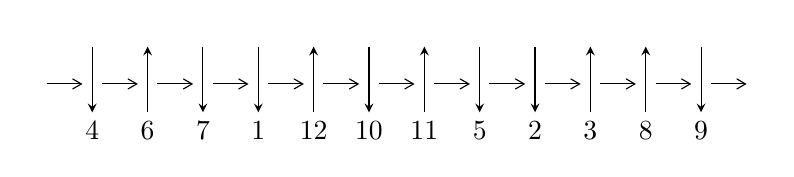
\begin{tikzpicture}[x=20pt, y=17pt]
	% nodes
	\node (C0) at (0, 0) {};
	\node (C1) at (1, 0) {};
	\node (C1U) at (1, +1) {};
	\node (C1D) at (1, -1) {4};

	\node (C2) at (2, 0) {};
	\node (C2U) at (2, +1) {};
	\node (C2D) at (2, -1) {6};

	\node (C3) at (3, 0) {};
	\node (C3U) at (3, +1) {};
	\node (C3D) at (3, -1) {7};

	\node (C4) at (4, 0) {};
	\node (C4U) at (4, +1) {};
	\node (C4D) at (4, -1) {1};

	\node (C5) at (5, 0) {};
	\node (C5U) at (5, +1) {};
	\node (C5D) at (5, -1) {12};

	\node (C6) at (6, 0) {};
	\node (C6U) at (6, +1) {};
	\node (C6D) at (6, -1) {10};

	\node (C7) at (7, 0) {};
	\node (C7U) at (7, +1) {};
	\node (C7D) at (7, -1) {11};

	\node (C8) at (8, 0) {};
	\node (C8U) at (8, +1) {};
	\node (C8D) at (8, -1) {5};

	\node (C9) at (9, 0) {};
	\node (C9U) at (9, +1) {};
	\node (C9D) at (9, -1) {2};

	\node (C10) at (10, 0) {};
	\node (C10U) at (10, +1) {};
	\node (C10D) at (10, -1) {3};

	\node (C11) at (11, 0) {};
	\node (C11U) at (11, +1) {};
	\node (C11D) at (11, -1) {8};

	\node (C12) at (12, 0) {};
	\node (C12U) at (12, +1) {};
	\node (C12D) at (12, -1) {9};
	\node (C13) at (13, 0) {};

	% arrows
	\draw[->,>={angle 60}]
	(C0) edge (C1) (C1) edge (C2) (C2) edge (C3) (C3) edge (C4) (C4) edge (C5) (C5) edge (C6) (C6) edge (C7) (C7) edge (C8) (C8) edge (C9) (C9) edge (C10) (C10) edge (C11) (C11) edge (C12) (C12) edge (C13) ;	\draw[->,>=stealth]
	(C1U) edge (C1D) (C2D) edge (C2U) (C3U) edge (C3D) (C4U) edge (C4D) (C5D) edge (C5U) (C6U) edge (C6D) (C7D) edge (C7U) (C8U) edge (C8D) (C9U) edge (C9D) (C10D) edge (C10U) (C11D) edge (C11U) (C12U) edge (C12D) ;
	\end{tikzpicture} \\
\hhline{~~} \\& 
\textbf{Solving Sequence} \\ \cline{2-2} 
 &
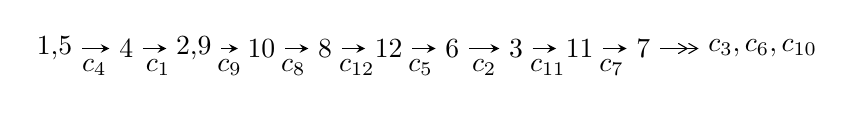
\begin{tikzpicture}[x=23pt, y=7pt]
	% node
	\node (A0) at (-1/8, 0) {1,5};
	\node (A1) at (1, 0) {4};
	\node (A2) at (33/16, 0) {2,9};
	\node (A3) at (25/8, 0) {10};
	\node (A4) at (33/8, 0) {8};
	\node (A5) at (41/8, 0) {12};
	\node (A6) at (49/8, 0) {6};
	\node (A7) at (57/8, 0) {3};
	\node (A8) at (65/8, 0) {11};
	\node (A9) at (73/8, 0) {7};
	\node (C1) at (1/2, -1) {$c_{4}$};
	\node (C2) at (3/2, -1) {$c_{1}$};
	\node (C3) at (21/8, -1) {$c_{9}$};
	\node (C4) at (29/8, -1) {$c_{8}$};
	\node (C5) at (37/8, -1) {$c_{12}$};
	\node (C6) at (45/8, -1) {$c_{5}$};
	\node (C7) at (53/8, -1) {$c_{2}$};
	\node (C8) at (61/8, -1) {$c_{11}$};
	\node (C9) at (69/8, -1) {$c_{7}$};
	\node (A10) at (11, 0) {$c_{3},c_{6},c_{10}$};

	% edge
	\draw[->,>=stealth]	
	(A0) edge (A1) (A1) edge (A2) (A2) edge (A3) (A3) edge (A4) (A4) edge (A5) (A5) edge (A6) (A6) edge (A7) (A7) edge (A8) (A8) edge (A9) ;
	\draw[->>,>={angle 60}]	
	(A9) edge (A10);
\end{tikzpicture} \\ 

\end{tabular} \\

\footnotetext{
The image of knot diagram is generated by the software ``\textbf{Draw programme}" developed by Andrew Bartholomew(\url{http://www.layer8.co.uk/maths/draw/index.htm\#Running-draw}), where we modified some parts for our purpose(\url{https://github.com/CATsTAILs/LinksPainter}).
}\phantom \\ \newline 
\centering \textbf{Ideals for irreducible components\footnotemark of $X_{\text{par}}$} 
 
\begin{align*}
I^u_{1}&=\langle 
-1.23311\times10^{1321} u^{182}-1.04572\times10^{1322} u^{181}+\cdots+9.42107\times10^{1324} b+6.84728\times10^{1326},\\
\phantom{I^u_{1}}&\phantom{= \langle  }2.05752\times10^{1324} u^{182}-1.58554\times10^{1325} u^{181}+\cdots+4.70704\times10^{1327} a+3.38310\times10^{1329},\\
\phantom{I^u_{1}}&\phantom{= \langle  }u^{183}-4 u^{182}+\cdots-183798 u-52461\rangle \\
I^u_{2}&=\langle 
1.76355\times10^{53} u^{46}+1.58871\times10^{54} u^{45}+\cdots+8.44121\times10^{52} b+1.62815\times10^{54},\\
\phantom{I^u_{2}}&\phantom{= \langle  }-2.19349\times10^{53} u^{46}-1.93560\times10^{54} u^{45}+\cdots+1.20589\times10^{52} a-1.36685\times10^{54},\\
\phantom{I^u_{2}}&\phantom{= \langle  }u^{47}+9 u^{46}+\cdots+24 u+1\rangle \\
\\
\end{align*}
\raggedright * 2 irreducible components of $\dim_{\mathbb{C}}=0$, with total 230 representations.\\
\footnotetext{All coefficients of polynomials are rational numbers. But the coefficients are sometimes approximated in decimal forms when there is not enough margin.}
\newpage
\renewcommand{\arraystretch}{1}
\centering \section*{I. $I^u_{1}= \langle -1.23\times10^{1321} u^{182}-1.05\times10^{1322} u^{181}+\cdots+9.42\times10^{1324} b+6.85\times10^{1326},\;2.06\times10^{1324} u^{182}-1.59\times10^{1325} u^{181}+\cdots+4.71\times10^{1327} a+3.38\times10^{1329},\;u^{183}-4 u^{182}+\cdots-183798 u-52461 \rangle$}
\flushleft \textbf{(i) Arc colorings}\\
\begin{tabular}{m{7pt} m{180pt} m{7pt} m{180pt} }
\flushright $a_{1}=$&$\begin{pmatrix}0\\u\end{pmatrix}$ \\
\flushright $a_{5}=$&$\begin{pmatrix}1\\0\end{pmatrix}$ \\
\flushright $a_{4}=$&$\begin{pmatrix}1\\- u^2\end{pmatrix}$ \\
\flushright $a_{2}=$&$\begin{pmatrix}- u\\u^3+u\end{pmatrix}$ \\
\flushright $a_{9}=$&$\begin{pmatrix}-0.000437115 u^{182}+0.00336845 u^{181}+\cdots-250.884 u-71.8732\\0.000130888 u^{182}+0.00110998 u^{181}+\cdots-248.349 u-72.6805\end{pmatrix}$ \\
\flushright $a_{10}=$&$\begin{pmatrix}-0.000331403 u^{182}+0.00448532 u^{181}+\cdots-500.110 u-140.941\\0.0000835116 u^{182}+0.00156077 u^{181}+\cdots-287.666 u-84.3878\end{pmatrix}$ \\
\flushright $a_{8}=$&$\begin{pmatrix}-0.000306227 u^{182}+0.00447843 u^{181}+\cdots-499.233 u-144.554\\0.000130888 u^{182}+0.00110998 u^{181}+\cdots-248.349 u-72.6805\end{pmatrix}$ \\
\flushright $a_{12}=$&$\begin{pmatrix}-0.00347163 u^{182}+0.0110800 u^{181}+\cdots+602.397 u+123.260\\-0.00167816 u^{182}+0.00558788 u^{181}+\cdots+256.078 u+53.2486\end{pmatrix}$ \\
\flushright $a_{6}=$&$\begin{pmatrix}-0.00432757 u^{182}+0.0193125 u^{181}+\cdots-98.1824 u-70.2159\\-0.00251588 u^{182}+0.0123166 u^{181}+\cdots-224.975 u-97.0449\end{pmatrix}$ \\
\flushright $a_{3}=$&$\begin{pmatrix}-0.000725381 u^{182}+0.00428746 u^{181}+\cdots-247.036 u-92.9010\\-0.000269656 u^{182}+0.00213422 u^{181}+\cdots-237.320 u-81.4091\end{pmatrix}$ \\
\flushright $a_{11}=$&$\begin{pmatrix}-0.00444480 u^{182}+0.0143521 u^{181}+\cdots+796.155 u+173.803\\-0.00259495 u^{182}+0.00946862 u^{181}+\cdots+294.790 u+58.7802\end{pmatrix}$ \\
\flushright $a_{7}=$&$\begin{pmatrix}-0.00446128 u^{182}+0.0166268 u^{181}+\cdots+464.515 u+79.1026\\-0.00310175 u^{182}+0.0118779 u^{181}+\cdots+246.090 u+34.9016\end{pmatrix}$\\&\end{tabular}
\flushleft \textbf{(ii) Obstruction class $= -1$}\\~\\
\flushleft \textbf{(iii) Cusp Shapes $= 0.00341695 u^{182}-0.0213085 u^{181}+\cdots+1013.78 u+305.421$}\\~\\
\newpage\renewcommand{\arraystretch}{1}
\flushleft \textbf{(iv) u-Polynomials at the component}\newline \\
\begin{tabular}{m{50pt}|m{274pt}}
Crossings & \hspace{64pt}u-Polynomials at each crossing \\
\hline $$\begin{aligned}c_{1},c_{4}\end{aligned}$$&$\begin{aligned}
&u^{183}+4 u^{182}+\cdots-183798 u+52461
\end{aligned}$\\
\hline $$\begin{aligned}c_{2}\end{aligned}$$&$\begin{aligned}
&u^{183}-2 u^{182}+\cdots-318294 u-40021
\end{aligned}$\\
\hline $$\begin{aligned}c_{3}\end{aligned}$$&$\begin{aligned}
&u^{183}+u^{182}+\cdots+2518528 u-157696
\end{aligned}$\\
\hline $$\begin{aligned}c_{5}\end{aligned}$$&$\begin{aligned}
&u^{183}+2 u^{182}+\cdots-626724 u-79331
\end{aligned}$\\
\hline $$\begin{aligned}c_{6}\end{aligned}$$&$\begin{aligned}
&u^{183}-2 u^{182}+\cdots+1244 u+203
\end{aligned}$\\
\hline $$\begin{aligned}c_{7},c_{11}\end{aligned}$$&$\begin{aligned}
&u^{183}-3 u^{182}+\cdots-13392267 u-702451
\end{aligned}$\\
\hline $$\begin{aligned}c_{8}\end{aligned}$$&$\begin{aligned}
&7(7 u^{183}-18 u^{182}+\cdots+2.12491\times10^{7} u+234650)
\end{aligned}$\\
\hline $$\begin{aligned}c_{9}\end{aligned}$$&$\begin{aligned}
&7(7 u^{183}-34 u^{182}+\cdots+2.80348\times10^{7} u-1352596)
\end{aligned}$\\
\hline $$\begin{aligned}c_{10}\end{aligned}$$&$\begin{aligned}
&7(7 u^{183}+u^{182}+\cdots+354748 u+24677)
\end{aligned}$\\
\hline $$\begin{aligned}c_{12}\end{aligned}$$&$\begin{aligned}
&u^{183}- u^{182}+\cdots+9088 u-448
\end{aligned}$\\
\hline
\end{tabular}\\~\\
\newpage\renewcommand{\arraystretch}{1}
\flushleft \textbf{(v) Riley Polynomials at the component}\newline \\
\begin{tabular}{m{50pt}|m{274pt}}
Crossings & \hspace{64pt}Riley Polynomials at each crossing \\
\hline $$\begin{aligned}c_{1},c_{4}\end{aligned}$$&$\begin{aligned}
&y^{183}+142 y^{182}+\cdots-132303001266 y-2752156521
\end{aligned}$\\
\hline $$\begin{aligned}c_{2}\end{aligned}$$&$\begin{aligned}
&y^{183}+2 y^{182}+\cdots+214292514570 y-1601680441
\end{aligned}$\\
\hline $$\begin{aligned}c_{3}\end{aligned}$$&$\begin{aligned}
&y^{183}+57 y^{182}+\cdots-1746473320448 y-24868028416
\end{aligned}$\\
\hline $$\begin{aligned}c_{5}\end{aligned}$$&$\begin{aligned}
&y^{183}-20 y^{182}+\cdots+171767282162 y-6293407561
\end{aligned}$\\
\hline $$\begin{aligned}c_{6}\end{aligned}$$&$\begin{aligned}
&y^{183}-6 y^{182}+\cdots+3080998 y-41209
\end{aligned}$\\
\hline $$\begin{aligned}c_{7},c_{11}\end{aligned}$$&$\begin{aligned}
&y^{183}-151 y^{182}+\cdots+52196002203823 y-493437407401
\end{aligned}$\\
\hline $$\begin{aligned}c_{8}\end{aligned}$$&$\begin{aligned}
&49(49 y^{183}+3834 y^{182}+\cdots+5.29211\times10^{14} y-5.50606\times10^{10})
\end{aligned}$\\
\hline $$\begin{aligned}c_{9}\end{aligned}$$&$\begin{aligned}
&49\\
&\cdot(49 y^{183}-2136 y^{182}+\cdots+122950525332321 y-1829515939216)
\end{aligned}$\\
\hline $$\begin{aligned}c_{10}\end{aligned}$$&$\begin{aligned}
&49(49 y^{183}-2479 y^{182}+\cdots+5.75236\times10^{10} y-6.08954\times10^{8})
\end{aligned}$\\
\hline $$\begin{aligned}c_{12}\end{aligned}$$&$\begin{aligned}
&y^{183}+25 y^{182}+\cdots+604160 y-200704
\end{aligned}$\\
\hline
\end{tabular}\\~\\
\newpage\flushleft \textbf{(vi) Complex Volumes and Cusp Shapes}
$$\begin{array}{c|c|c}  
\text{Solutions to }I^u_{1}& \I (\text{vol} + \sqrt{-1}CS) & \text{Cusp shape}\\
 \hline 
\begin{aligned}
u &= \phantom{-}0.353361 + 0.935758 I \\
a &= \phantom{-}0.222524 + 0.249072 I \\
b &= -0.94781 + 1.58440 I\end{aligned}
 & \phantom{-}1.74024 - 1.78318 I & \phantom{-0.000000 } 0 \\ \hline\begin{aligned}
u &= \phantom{-}0.353361 - 0.935758 I \\
a &= \phantom{-}0.222524 - 0.249072 I \\
b &= -0.94781 - 1.58440 I\end{aligned}
 & \phantom{-}1.74024 + 1.78318 I & \phantom{-0.000000 } 0 \\ \hline\begin{aligned}
u &= -0.996758 + 0.017899 I \\
a &= \phantom{-}0.743697 - 0.766270 I \\
b &= -0.717105 + 1.009770 I\end{aligned}
 & \phantom{-}4.30464 + 7.27339 I & \phantom{-0.000000 } 0 \\ \hline\begin{aligned}
u &= -0.996758 - 0.017899 I \\
a &= \phantom{-}0.743697 + 0.766270 I \\
b &= -0.717105 - 1.009770 I\end{aligned}
 & \phantom{-}4.30464 - 7.27339 I & \phantom{-0.000000 } 0 \\ \hline\begin{aligned}
u &= -1.005900 + 0.068998 I \\
a &= \phantom{-}1.010940 - 0.591258 I \\
b &= -0.755267 + 0.718964 I\end{aligned}
 & -3.33360 + 9.53239 I & \phantom{-0.000000 } 0 \\ \hline\begin{aligned}
u &= -1.005900 - 0.068998 I \\
a &= \phantom{-}1.010940 + 0.591258 I \\
b &= -0.755267 - 0.718964 I\end{aligned}
 & -3.33360 - 9.53239 I & \phantom{-0.000000 } 0 \\ \hline\begin{aligned}
u &= -0.878637 + 0.509873 I \\
a &= -0.346505 - 0.879630 I \\
b &= \phantom{-}0.594251 + 0.741620 I\end{aligned}
 & -1.96779 - 0.01153 I & \phantom{-0.000000 } 0 \\ \hline\begin{aligned}
u &= -0.878637 - 0.509873 I \\
a &= -0.346505 + 0.879630 I \\
b &= \phantom{-}0.594251 - 0.741620 I\end{aligned}
 & -1.96779 + 0.01153 I & \phantom{-0.000000 } 0 \\ \hline\begin{aligned}
u &= -0.263132 + 0.999119 I \\
a &= \phantom{-}0.362798 + 0.310372 I \\
b &= -1.81846 + 0.02694 I\end{aligned}
 & \phantom{-}4.99563 + 4.29408 I & \phantom{-0.000000 } 0 \\ \hline\begin{aligned}
u &= -0.263132 - 0.999119 I \\
a &= \phantom{-}0.362798 - 0.310372 I \\
b &= -1.81846 - 0.02694 I\end{aligned}
 & \phantom{-}4.99563 - 4.29408 I & \phantom{-0.000000 } 0\\
 \hline 
 \end{array}$$\newpage$$\begin{array}{c|c|c}  
\text{Solutions to }I^u_{1}& \I (\text{vol} + \sqrt{-1}CS) & \text{Cusp shape}\\
 \hline 
\begin{aligned}
u &= \phantom{-}0.946198 + 0.066457 I \\
a &= \phantom{-}0.952445 + 0.634107 I \\
b &= -0.600046 - 1.133960 I\end{aligned}
 & \phantom{-}2.76487 - 5.29634 I & \phantom{-0.000000 } 0 \\ \hline\begin{aligned}
u &= \phantom{-}0.946198 - 0.066457 I \\
a &= \phantom{-}0.952445 - 0.634107 I \\
b &= -0.600046 + 1.133960 I\end{aligned}
 & \phantom{-}2.76487 + 5.29634 I & \phantom{-0.000000 } 0 \\ \hline\begin{aligned}
u &= \phantom{-}0.366480 + 0.990925 I \\
a &= \phantom{-}1.57808 - 0.46897 I \\
b &= -0.497082 - 0.728812 I\end{aligned}
 & -0.25857 - 4.52320 I & \phantom{-0.000000 } 0 \\ \hline\begin{aligned}
u &= \phantom{-}0.366480 - 0.990925 I \\
a &= \phantom{-}1.57808 + 0.46897 I \\
b &= -0.497082 + 0.728812 I\end{aligned}
 & -0.25857 + 4.52320 I & \phantom{-0.000000 } 0 \\ \hline\begin{aligned}
u &= \phantom{-}1.057230 + 0.043906 I \\
a &= -0.762989 - 0.253049 I \\
b &= \phantom{-}0.848577 + 0.622499 I\end{aligned}
 & -3.58567 - 1.82509 I & \phantom{-0.000000 } 0 \\ \hline\begin{aligned}
u &= \phantom{-}1.057230 - 0.043906 I \\
a &= -0.762989 + 0.253049 I \\
b &= \phantom{-}0.848577 - 0.622499 I\end{aligned}
 & -3.58567 + 1.82509 I & \phantom{-0.000000 } 0 \\ \hline\begin{aligned}
u &= -0.220734 + 0.913464 I \\
a &= -0.52460 - 1.34256 I \\
b &= \phantom{-}0.397501 - 1.207380 I\end{aligned}
 & -0.85432 + 4.03337 I & \phantom{-0.000000 } 0 \\ \hline\begin{aligned}
u &= -0.220734 - 0.913464 I \\
a &= -0.52460 + 1.34256 I \\
b &= \phantom{-}0.397501 + 1.207380 I\end{aligned}
 & -0.85432 - 4.03337 I & \phantom{-0.000000 } 0 \\ \hline\begin{aligned}
u &= \phantom{-}1.048520 + 0.168591 I \\
a &= \phantom{-}0.963110 + 0.345834 I \\
b &= -0.673624 - 0.515132 I\end{aligned}
 & -3.37727 - 2.33210 I & \phantom{-0.000000 } 0 \\ \hline\begin{aligned}
u &= \phantom{-}1.048520 - 0.168591 I \\
a &= \phantom{-}0.963110 - 0.345834 I \\
b &= -0.673624 + 0.515132 I\end{aligned}
 & -3.37727 + 2.33210 I & \phantom{-0.000000 } 0\\
 \hline 
 \end{array}$$\newpage$$\begin{array}{c|c|c}  
\text{Solutions to }I^u_{1}& \I (\text{vol} + \sqrt{-1}CS) & \text{Cusp shape}\\
 \hline 
\begin{aligned}
u &= \phantom{-}0.218643 + 0.911081 I \\
a &= \phantom{-}0.460486 + 0.578131 I \\
b &= -0.325169 + 1.101020 I\end{aligned}
 & \phantom{-}1.79037 - 1.85431 I & \phantom{-0.000000 } 0 \\ \hline\begin{aligned}
u &= \phantom{-}0.218643 - 0.911081 I \\
a &= \phantom{-}0.460486 - 0.578131 I \\
b &= -0.325169 - 1.101020 I\end{aligned}
 & \phantom{-}1.79037 + 1.85431 I & \phantom{-0.000000 } 0 \\ \hline\begin{aligned}
u &= -0.234778 + 0.906789 I \\
a &= \phantom{-}1.66370 - 0.15218 I \\
b &= -0.569059 + 0.991582 I\end{aligned}
 & \phantom{-}6.87653 + 1.24248 I & \phantom{-0.000000 } 0 \\ \hline\begin{aligned}
u &= -0.234778 - 0.906789 I \\
a &= \phantom{-}1.66370 + 0.15218 I \\
b &= -0.569059 - 0.991582 I\end{aligned}
 & \phantom{-}6.87653 - 1.24248 I & \phantom{-0.000000 } 0 \\ \hline\begin{aligned}
u &= -0.130337 + 1.056720 I \\
a &= \phantom{-}1.24837 + 0.79566 I \\
b &= -0.64933 + 1.40979 I\end{aligned}
 & \phantom{-}7.56133 + 5.13956 I & \phantom{-0.000000 } 0 \\ \hline\begin{aligned}
u &= -0.130337 - 1.056720 I \\
a &= \phantom{-}1.24837 - 0.79566 I \\
b &= -0.64933 - 1.40979 I\end{aligned}
 & \phantom{-}7.56133 - 5.13956 I & \phantom{-0.000000 } 0 \\ \hline\begin{aligned}
u &= \phantom{-}0.102430 + 1.061440 I \\
a &= -0.129601 - 0.937600 I \\
b &= \phantom{-}0.25067 - 2.05061 I\end{aligned}
 & \phantom{-}2.55597 - 0.05704 I & \phantom{-0.000000 } 0 \\ \hline\begin{aligned}
u &= \phantom{-}0.102430 - 1.061440 I \\
a &= -0.129601 + 0.937600 I \\
b &= \phantom{-}0.25067 + 2.05061 I\end{aligned}
 & \phantom{-}2.55597 + 0.05704 I & \phantom{-0.000000 } 0 \\ \hline\begin{aligned}
u &= -0.081149 + 1.064730 I \\
a &= \phantom{-}0.251050 + 1.350510 I \\
b &= -0.15888 + 1.75753 I\end{aligned}
 & \phantom{-}1.88430 + 6.51448 I & \phantom{-0.000000 } 0 \\ \hline\begin{aligned}
u &= -0.081149 - 1.064730 I \\
a &= \phantom{-}0.251050 - 1.350510 I \\
b &= -0.15888 - 1.75753 I\end{aligned}
 & \phantom{-}1.88430 - 6.51448 I & \phantom{-0.000000 } 0\\
 \hline 
 \end{array}$$\newpage$$\begin{array}{c|c|c}  
\text{Solutions to }I^u_{1}& \I (\text{vol} + \sqrt{-1}CS) & \text{Cusp shape}\\
 \hline 
\begin{aligned}
u &= -0.788921 + 0.480921 I \\
a &= -0.692194 - 0.773701 I \\
b &= \phantom{-}1.07762 - 0.95301 I\end{aligned}
 & \phantom{-}2.43066 - 7.71293 I & \phantom{-0.000000 } 0 \\ \hline\begin{aligned}
u &= -0.788921 - 0.480921 I \\
a &= -0.692194 + 0.773701 I \\
b &= \phantom{-}1.07762 + 0.95301 I\end{aligned}
 & \phantom{-}2.43066 + 7.71293 I & \phantom{-0.000000 } 0 \\ \hline\begin{aligned}
u &= \phantom{-}0.716335 + 0.569837 I \\
a &= -1.027840 + 0.274184 I \\
b &= \phantom{-}0.695669 + 1.130800 I\end{aligned}
 & -2.10543 - 4.06058 I & \phantom{-0.000000 } 0 \\ \hline\begin{aligned}
u &= \phantom{-}0.716335 - 0.569837 I \\
a &= -1.027840 - 0.274184 I \\
b &= \phantom{-}0.695669 - 1.130800 I\end{aligned}
 & -2.10543 + 4.06058 I & \phantom{-0.000000 } 0 \\ \hline\begin{aligned}
u &= \phantom{-}0.047368 + 1.087940 I \\
a &= -1.128930 - 0.832709 I \\
b &= \phantom{-}0.611281 - 1.044630 I\end{aligned}
 & \phantom{-}2.46520 + 1.29570 I & \phantom{-0.000000 } 0 \\ \hline\begin{aligned}
u &= \phantom{-}0.047368 - 1.087940 I \\
a &= -1.128930 + 0.832709 I \\
b &= \phantom{-}0.611281 + 1.044630 I\end{aligned}
 & \phantom{-}2.46520 - 1.29570 I & \phantom{-0.000000 } 0 \\ \hline\begin{aligned}
u &= -0.939429 + 0.586393 I \\
a &= \phantom{-}0.404949 - 0.510478 I \\
b &= -0.128717 + 0.660503 I\end{aligned}
 & \phantom{-}0.98787 - 2.24903 I & \phantom{-0.000000 } 0 \\ \hline\begin{aligned}
u &= -0.939429 - 0.586393 I \\
a &= \phantom{-}0.404949 + 0.510478 I \\
b &= -0.128717 - 0.660503 I\end{aligned}
 & \phantom{-}0.98787 + 2.24903 I & \phantom{-0.000000 } 0 \\ \hline\begin{aligned}
u &= \phantom{-}0.300353 + 0.838277 I \\
a &= \phantom{-}1.68395 + 0.66185 I \\
b &= -0.614944 - 0.759039 I\end{aligned}
 & \phantom{-}5.99125 - 3.44755 I & \phantom{-0.000000 } 0 \\ \hline\begin{aligned}
u &= \phantom{-}0.300353 - 0.838277 I \\
a &= \phantom{-}1.68395 - 0.66185 I \\
b &= -0.614944 + 0.759039 I\end{aligned}
 & \phantom{-}5.99125 + 3.44755 I & \phantom{-0.000000 } 0\\
 \hline 
 \end{array}$$\newpage$$\begin{array}{c|c|c}  
\text{Solutions to }I^u_{1}& \I (\text{vol} + \sqrt{-1}CS) & \text{Cusp shape}\\
 \hline 
\begin{aligned}
u &= \phantom{-}0.887469\phantom{ +0.000000I} \\
a &= \phantom{-}0.549715\phantom{ +0.000000I} \\
b &= \phantom{-}0.0101625\phantom{ +0.000000I}\end{aligned}
 & -1.71845\phantom{ +0.000000I} & \phantom{-0.000000 } 0 \\ \hline\begin{aligned}
u &= \phantom{-}0.083492 + 1.116180 I \\
a &= \phantom{-}0.777356 - 0.469521 I \\
b &= -1.20757 - 1.67865 I\end{aligned}
 & \phantom{-}7.44089 - 4.05881 I & \phantom{-0.000000 } 0 \\ \hline\begin{aligned}
u &= \phantom{-}0.083492 - 1.116180 I \\
a &= \phantom{-}0.777356 + 0.469521 I \\
b &= -1.20757 + 1.67865 I\end{aligned}
 & \phantom{-}7.44089 + 4.05881 I & \phantom{-0.000000 } 0 \\ \hline\begin{aligned}
u &= -0.326054 + 1.075000 I \\
a &= \phantom{-}1.32904 + 0.91384 I \\
b &= -0.487753 + 0.736488 I\end{aligned}
 & -0.19557 - 1.78627 I & \phantom{-0.000000 } 0 \\ \hline\begin{aligned}
u &= -0.326054 - 1.075000 I \\
a &= \phantom{-}1.32904 - 0.91384 I \\
b &= -0.487753 - 0.736488 I\end{aligned}
 & -0.19557 + 1.78627 I & \phantom{-0.000000 } 0 \\ \hline\begin{aligned}
u &= \phantom{-}0.798489 + 0.356338 I \\
a &= \phantom{-}0.695522 - 0.796183 I \\
b &= -0.246041 + 0.425888 I\end{aligned}
 & -2.16763 + 0.10355 I & \phantom{-0.000000 } 0 \\ \hline\begin{aligned}
u &= \phantom{-}0.798489 - 0.356338 I \\
a &= \phantom{-}0.695522 + 0.796183 I \\
b &= -0.246041 - 0.425888 I\end{aligned}
 & -2.16763 - 0.10355 I & \phantom{-0.000000 } 0 \\ \hline\begin{aligned}
u &= -0.073928 + 1.131220 I \\
a &= -1.59262 + 0.61619 I \\
b &= \phantom{-}0.529033 + 0.585016 I\end{aligned}
 & \phantom{-}2.24288 + 4.34518 I & \phantom{-0.000000 } 0 \\ \hline\begin{aligned}
u &= -0.073928 - 1.131220 I \\
a &= -1.59262 - 0.61619 I \\
b &= \phantom{-}0.529033 - 0.585016 I\end{aligned}
 & \phantom{-}2.24288 - 4.34518 I & \phantom{-0.000000 } 0 \\ \hline\begin{aligned}
u &= \phantom{-}0.004398 + 1.140070 I \\
a &= -1.49668 - 0.93345 I \\
b &= \phantom{-}0.009395 - 0.924953 I\end{aligned}
 & \phantom{-}8.34632 - 0.46353 I & \phantom{-0.000000 } 0\\
 \hline 
 \end{array}$$\newpage$$\begin{array}{c|c|c}  
\text{Solutions to }I^u_{1}& \I (\text{vol} + \sqrt{-1}CS) & \text{Cusp shape}\\
 \hline 
\begin{aligned}
u &= \phantom{-}0.004398 - 1.140070 I \\
a &= -1.49668 + 0.93345 I \\
b &= \phantom{-}0.009395 + 0.924953 I\end{aligned}
 & \phantom{-}8.34632 + 0.46353 I & \phantom{-0.000000 } 0 \\ \hline\begin{aligned}
u &= -0.269624 + 1.111210 I \\
a &= \phantom{-}0.338858 + 0.100705 I \\
b &= -1.35123 - 0.91146 I\end{aligned}
 & \phantom{-}0.41612 + 7.30003 I & \phantom{-0.000000 } 0 \\ \hline\begin{aligned}
u &= -0.269624 - 1.111210 I \\
a &= \phantom{-}0.338858 - 0.100705 I \\
b &= -1.35123 + 0.91146 I\end{aligned}
 & \phantom{-}0.41612 - 7.30003 I & \phantom{-0.000000 } 0 \\ \hline\begin{aligned}
u &= \phantom{-}0.536428 + 0.653241 I \\
a &= -0.141720 + 0.153670 I \\
b &= \phantom{-}0.916447 - 0.227859 I\end{aligned}
 & -1.77674 - 0.85721 I & \phantom{-0.000000 } 0 \\ \hline\begin{aligned}
u &= \phantom{-}0.536428 - 0.653241 I \\
a &= -0.141720 - 0.153670 I \\
b &= \phantom{-}0.916447 + 0.227859 I\end{aligned}
 & -1.77674 + 0.85721 I & \phantom{-0.000000 } 0 \\ \hline\begin{aligned}
u &= -0.484167 + 1.050870 I \\
a &= -0.457670 - 0.232103 I \\
b &= \phantom{-}1.92140 + 0.11159 I\end{aligned}
 & \phantom{-}4.17759 + 12.48690 I & \phantom{-0.000000 } 0 \\ \hline\begin{aligned}
u &= -0.484167 - 1.050870 I \\
a &= -0.457670 + 0.232103 I \\
b &= \phantom{-}1.92140 - 0.11159 I\end{aligned}
 & \phantom{-}4.17759 - 12.48690 I & \phantom{-0.000000 } 0 \\ \hline\begin{aligned}
u &= -0.045426 + 1.157010 I \\
a &= -1.35060 + 1.31535 I \\
b &= -0.025880 + 0.733816 I\end{aligned}
 & \phantom{-}8.21427 + 2.89848 I & \phantom{-0.000000 } 0 \\ \hline\begin{aligned}
u &= -0.045426 - 1.157010 I \\
a &= -1.35060 - 1.31535 I \\
b &= -0.025880 - 0.733816 I\end{aligned}
 & \phantom{-}8.21427 - 2.89848 I & \phantom{-0.000000 } 0 \\ \hline\begin{aligned}
u &= \phantom{-}0.422818 + 0.724471 I \\
a &= -0.766881 - 0.223474 I \\
b &= \phantom{-}1.45001 - 1.15461 I\end{aligned}
 & \phantom{-}1.88033 - 1.35372 I & \phantom{-0.000000 } 0\\
 \hline 
 \end{array}$$\newpage$$\begin{array}{c|c|c}  
\text{Solutions to }I^u_{1}& \I (\text{vol} + \sqrt{-1}CS) & \text{Cusp shape}\\
 \hline 
\begin{aligned}
u &= \phantom{-}0.422818 - 0.724471 I \\
a &= -0.766881 + 0.223474 I \\
b &= \phantom{-}1.45001 + 1.15461 I\end{aligned}
 & \phantom{-}1.88033 + 1.35372 I & \phantom{-0.000000 } 0 \\ \hline\begin{aligned}
u &= \phantom{-}0.831342\phantom{ +0.000000I} \\
a &= \phantom{-}1.33235\phantom{ +0.000000I} \\
b &= -0.948288\phantom{ +0.000000I}\end{aligned}
 & -0.483949\phantom{ +0.000000I} & \phantom{-0.000000 } 0 \\ \hline\begin{aligned}
u &= \phantom{-}0.028257 + 1.174870 I \\
a &= -0.261634 + 0.021606 I \\
b &= \phantom{-}0.963858 + 0.991946 I\end{aligned}
 & \phantom{-}2.99812 - 1.63320 I & \phantom{-0.000000 } 0 \\ \hline\begin{aligned}
u &= \phantom{-}0.028257 - 1.174870 I \\
a &= -0.261634 - 0.021606 I \\
b &= \phantom{-}0.963858 - 0.991946 I\end{aligned}
 & \phantom{-}2.99812 + 1.63320 I & \phantom{-0.000000 } 0 \\ \hline\begin{aligned}
u &= -0.458504 + 1.089010 I \\
a &= -1.297240 - 0.413359 I \\
b &= \phantom{-}0.777085 - 1.091510 I\end{aligned}
 & -0.02440 + 4.89286 I & \phantom{-0.000000 } 0 \\ \hline\begin{aligned}
u &= -0.458504 - 1.089010 I \\
a &= -1.297240 + 0.413359 I \\
b &= \phantom{-}0.777085 + 1.091510 I\end{aligned}
 & -0.02440 - 4.89286 I & \phantom{-0.000000 } 0 \\ \hline\begin{aligned}
u &= \phantom{-}0.849201 + 0.825469 I \\
a &= \phantom{-}0.552684 - 0.426529 I \\
b &= -1.31940 - 0.63872 I\end{aligned}
 & \phantom{-}0.09413 - 3.09571 I & \phantom{-0.000000 } 0 \\ \hline\begin{aligned}
u &= \phantom{-}0.849201 - 0.825469 I \\
a &= \phantom{-}0.552684 + 0.426529 I \\
b &= -1.31940 + 0.63872 I\end{aligned}
 & \phantom{-}0.09413 + 3.09571 I & \phantom{-0.000000 } 0 \\ \hline\begin{aligned}
u &= -0.070119 + 1.205630 I \\
a &= -0.980071 - 0.294533 I \\
b &= -0.113218 - 0.931316 I\end{aligned}
 & \phantom{-}8.07248 - 3.44277 I & \phantom{-0.000000 } 0 \\ \hline\begin{aligned}
u &= -0.070119 - 1.205630 I \\
a &= -0.980071 + 0.294533 I \\
b &= -0.113218 + 0.931316 I\end{aligned}
 & \phantom{-}8.07248 + 3.44277 I & \phantom{-0.000000 } 0\\
 \hline 
 \end{array}$$\newpage$$\begin{array}{c|c|c}  
\text{Solutions to }I^u_{1}& \I (\text{vol} + \sqrt{-1}CS) & \text{Cusp shape}\\
 \hline 
\begin{aligned}
u &= -0.190972 + 1.193950 I \\
a &= \phantom{-}1.08866 - 1.22515 I \\
b &= \phantom{-}0.081944 - 0.832532 I\end{aligned}
 & \phantom{-}7.83745 + 11.70160 I & \phantom{-0.000000 } 0 \\ \hline\begin{aligned}
u &= -0.190972 - 1.193950 I \\
a &= \phantom{-}1.08866 + 1.22515 I \\
b &= \phantom{-}0.081944 + 0.832532 I\end{aligned}
 & \phantom{-}7.83745 - 11.70160 I & \phantom{-0.000000 } 0 \\ \hline\begin{aligned}
u &= \phantom{-}0.368971 + 1.165730 I \\
a &= \phantom{-}0.630338 - 0.408816 I \\
b &= -1.027180 - 0.081457 I\end{aligned}
 & \phantom{-}3.11301 - 4.28028 I & \phantom{-0.000000 } 0 \\ \hline\begin{aligned}
u &= \phantom{-}0.368971 - 1.165730 I \\
a &= \phantom{-}0.630338 + 0.408816 I \\
b &= -1.027180 + 0.081457 I\end{aligned}
 & \phantom{-}3.11301 + 4.28028 I & \phantom{-0.000000 } 0 \\ \hline\begin{aligned}
u &= -0.244356 + 0.737492 I \\
a &= \phantom{-}0.108667 + 0.550986 I \\
b &= -0.364932 - 1.178350 I\end{aligned}
 & \phantom{-}0.96823 - 5.42523 I & \phantom{-0.000000 } 0 \\ \hline\begin{aligned}
u &= -0.244356 - 0.737492 I \\
a &= \phantom{-}0.108667 - 0.550986 I \\
b &= -0.364932 + 1.178350 I\end{aligned}
 & \phantom{-}0.96823 + 5.42523 I & \phantom{-0.000000 } 0 \\ \hline\begin{aligned}
u &= -0.083731 + 1.247490 I \\
a &= -0.406869 + 1.134010 I \\
b &= -0.230124 + 0.845856 I\end{aligned}
 & \phantom{-}7.69278 + 0.35419 I & \phantom{-0.000000 } 0 \\ \hline\begin{aligned}
u &= -0.083731 - 1.247490 I \\
a &= -0.406869 - 1.134010 I \\
b &= -0.230124 - 0.845856 I\end{aligned}
 & \phantom{-}7.69278 - 0.35419 I & \phantom{-0.000000 } 0 \\ \hline\begin{aligned}
u &= \phantom{-}0.463139 + 0.589493 I \\
a &= \phantom{-}0.12131 + 1.53874 I \\
b &= \phantom{-}0.343879 + 0.860642 I\end{aligned}
 & \phantom{-}1.81954 - 2.23994 I & \phantom{-0.000000 } 0 \\ \hline\begin{aligned}
u &= \phantom{-}0.463139 - 0.589493 I \\
a &= \phantom{-}0.12131 - 1.53874 I \\
b &= \phantom{-}0.343879 - 0.860642 I\end{aligned}
 & \phantom{-}1.81954 + 2.23994 I & \phantom{-0.000000 } 0\\
 \hline 
 \end{array}$$\newpage$$\begin{array}{c|c|c}  
\text{Solutions to }I^u_{1}& \I (\text{vol} + \sqrt{-1}CS) & \text{Cusp shape}\\
 \hline 
\begin{aligned}
u &= \phantom{-}0.155664 + 1.251670 I \\
a &= \phantom{-}1.061570 - 0.317033 I \\
b &= -1.010970 - 0.816892 I\end{aligned}
 & \phantom{-}4.45230 - 5.21175 I & \phantom{-0.000000 } 0 \\ \hline\begin{aligned}
u &= \phantom{-}0.155664 - 1.251670 I \\
a &= \phantom{-}1.061570 + 0.317033 I \\
b &= -1.010970 + 0.816892 I\end{aligned}
 & \phantom{-}4.45230 + 5.21175 I & \phantom{-0.000000 } 0 \\ \hline\begin{aligned}
u &= -1.190140 + 0.438550 I \\
a &= -0.512550 + 0.493114 I \\
b &= \phantom{-}0.770570 - 0.854996 I\end{aligned}
 & \phantom{-}4.52957 - 3.86574 I & \phantom{-0.000000 } 0 \\ \hline\begin{aligned}
u &= -1.190140 - 0.438550 I \\
a &= -0.512550 - 0.493114 I \\
b &= \phantom{-}0.770570 + 0.854996 I\end{aligned}
 & \phantom{-}4.52957 + 3.86574 I & \phantom{-0.000000 } 0 \\ \hline\begin{aligned}
u &= -0.286880 + 1.240540 I \\
a &= \phantom{-}0.959494 + 0.261179 I \\
b &= -0.601745 + 1.060420 I\end{aligned}
 & \phantom{-}6.22217 + 0.94119 I & \phantom{-0.000000 } 0 \\ \hline\begin{aligned}
u &= -0.286880 - 1.240540 I \\
a &= \phantom{-}0.959494 - 0.261179 I \\
b &= -0.601745 - 1.060420 I\end{aligned}
 & \phantom{-}6.22217 - 0.94119 I & \phantom{-0.000000 } 0 \\ \hline\begin{aligned}
u &= -0.264929 + 1.260310 I \\
a &= -1.163140 - 0.628802 I \\
b &= \phantom{-}0.895777 - 0.921002 I\end{aligned}
 & \phantom{-}2.82705 + 5.02590 I & \phantom{-0.000000 } 0 \\ \hline\begin{aligned}
u &= -0.264929 - 1.260310 I \\
a &= -1.163140 + 0.628802 I \\
b &= \phantom{-}0.895777 + 0.921002 I\end{aligned}
 & \phantom{-}2.82705 - 5.02590 I & \phantom{-0.000000 } 0 \\ \hline\begin{aligned}
u &= \phantom{-}0.206855 + 1.281810 I \\
a &= \phantom{-}0.849259 + 1.000950 I \\
b &= -0.011487 + 0.895548 I\end{aligned}
 & \phantom{-}5.91223 - 3.80922 I & \phantom{-0.000000 } 0 \\ \hline\begin{aligned}
u &= \phantom{-}0.206855 - 1.281810 I \\
a &= \phantom{-}0.849259 - 1.000950 I \\
b &= -0.011487 - 0.895548 I\end{aligned}
 & \phantom{-}5.91223 + 3.80922 I & \phantom{-0.000000 } 0\\
 \hline 
 \end{array}$$\newpage$$\begin{array}{c|c|c}  
\text{Solutions to }I^u_{1}& \I (\text{vol} + \sqrt{-1}CS) & \text{Cusp shape}\\
 \hline 
\begin{aligned}
u &= \phantom{-}0.656234 + 1.121240 I \\
a &= \phantom{-}0.464258 - 0.265021 I \\
b &= -0.543883 - 0.357689 I\end{aligned}
 & -0.45448 - 3.59651 I & \phantom{-0.000000 } 0 \\ \hline\begin{aligned}
u &= \phantom{-}0.656234 - 1.121240 I \\
a &= \phantom{-}0.464258 + 0.265021 I \\
b &= -0.543883 + 0.357689 I\end{aligned}
 & -0.45448 + 3.59651 I & \phantom{-0.000000 } 0 \\ \hline\begin{aligned}
u &= -0.691619 + 0.056259 I \\
a &= \phantom{-}0.233198 + 1.275080 I \\
b &= -0.566991 - 0.939656 I\end{aligned}
 & \phantom{-}5.89009 - 2.09906 I & \phantom{-0.000000 } 0 \\ \hline\begin{aligned}
u &= -0.691619 - 0.056259 I \\
a &= \phantom{-}0.233198 - 1.275080 I \\
b &= -0.566991 + 0.939656 I\end{aligned}
 & \phantom{-}5.89009 + 2.09906 I & \phantom{-0.000000 } 0 \\ \hline\begin{aligned}
u &= \phantom{-}1.293840 + 0.185622 I \\
a &= \phantom{-}0.555880 + 0.262877 I \\
b &= -0.957850 - 1.029210 I\end{aligned}
 & \phantom{-}1.05501 - 4.51121 I & \phantom{-0.000000 } 0 \\ \hline\begin{aligned}
u &= \phantom{-}1.293840 - 0.185622 I \\
a &= \phantom{-}0.555880 - 0.262877 I \\
b &= -0.957850 + 1.029210 I\end{aligned}
 & \phantom{-}1.05501 + 4.51121 I & \phantom{-0.000000 } 0 \\ \hline\begin{aligned}
u &= -0.198799 + 1.294160 I \\
a &= -1.40590 - 0.71544 I \\
b &= \phantom{-}0.697979 - 0.497053 I\end{aligned}
 & \phantom{-}2.00407 + 5.44742 I & \phantom{-0.000000 } 0 \\ \hline\begin{aligned}
u &= -0.198799 - 1.294160 I \\
a &= -1.40590 + 0.71544 I \\
b &= \phantom{-}0.697979 + 0.497053 I\end{aligned}
 & \phantom{-}2.00407 - 5.44742 I & \phantom{-0.000000 } 0 \\ \hline\begin{aligned}
u &= \phantom{-}0.178195 + 1.312730 I \\
a &= -0.231596 + 0.088504 I \\
b &= -0.190463 + 1.292530 I\end{aligned}
 & \phantom{-}6.87494 + 1.26054 I & \phantom{-0.000000 } 0 \\ \hline\begin{aligned}
u &= \phantom{-}0.178195 - 1.312730 I \\
a &= -0.231596 - 0.088504 I \\
b &= -0.190463 - 1.292530 I\end{aligned}
 & \phantom{-}6.87494 - 1.26054 I & \phantom{-0.000000 } 0\\
 \hline 
 \end{array}$$\newpage$$\begin{array}{c|c|c}  
\text{Solutions to }I^u_{1}& \I (\text{vol} + \sqrt{-1}CS) & \text{Cusp shape}\\
 \hline 
\begin{aligned}
u &= \phantom{-}0.493813 + 1.233590 I \\
a &= -1.112530 - 0.274480 I \\
b &= -0.066058 + 0.814084 I\end{aligned}
 & \phantom{-}7.85689 - 0.20204 I & \phantom{-0.000000 } 0 \\ \hline\begin{aligned}
u &= \phantom{-}0.493813 - 1.233590 I \\
a &= -1.112530 + 0.274480 I \\
b &= -0.066058 - 0.814084 I\end{aligned}
 & \phantom{-}7.85689 + 0.20204 I & \phantom{-0.000000 } 0 \\ \hline\begin{aligned}
u &= \phantom{-}0.829346 + 1.076770 I \\
a &= -1.046620 - 0.031456 I \\
b &= \phantom{-}0.849883 + 1.096060 I\end{aligned}
 & \phantom{-}2.89341 - 8.99267 I & \phantom{-0.000000 } 0 \\ \hline\begin{aligned}
u &= \phantom{-}0.829346 - 1.076770 I \\
a &= -1.046620 + 0.031456 I \\
b &= \phantom{-}0.849883 - 1.096060 I\end{aligned}
 & \phantom{-}2.89341 + 8.99267 I & \phantom{-0.000000 } 0 \\ \hline\begin{aligned}
u &= \phantom{-}0.308675 + 1.328600 I \\
a &= \phantom{-}0.884486 - 0.411016 I \\
b &= -0.508356 - 0.440787 I\end{aligned}
 & \phantom{-}3.21363 - 3.91201 I & \phantom{-0.000000 } 0 \\ \hline\begin{aligned}
u &= \phantom{-}0.308675 - 1.328600 I \\
a &= \phantom{-}0.884486 + 0.411016 I \\
b &= -0.508356 + 0.440787 I\end{aligned}
 & \phantom{-}3.21363 + 3.91201 I & \phantom{-0.000000 } 0 \\ \hline\begin{aligned}
u &= -1.368980 + 0.132745 I \\
a &= -0.637508 + 0.441709 I \\
b &= \phantom{-}0.828747 - 0.970265 I\end{aligned}
 & \phantom{-}2.7675 + 14.4661 I & \phantom{-0.000000 } 0 \\ \hline\begin{aligned}
u &= -1.368980 - 0.132745 I \\
a &= -0.637508 - 0.441709 I \\
b &= \phantom{-}0.828747 + 0.970265 I\end{aligned}
 & \phantom{-}2.7675 - 14.4661 I & \phantom{-0.000000 } 0 \\ \hline\begin{aligned}
u &= \phantom{-}0.523848 + 1.278390 I \\
a &= -0.391147 + 0.071671 I \\
b &= \phantom{-}0.842500 + 0.277597 I\end{aligned}
 & \phantom{-}0.19061 - 3.72591 I & \phantom{-0.000000 } 0 \\ \hline\begin{aligned}
u &= \phantom{-}0.523848 - 1.278390 I \\
a &= -0.391147 - 0.071671 I \\
b &= \phantom{-}0.842500 - 0.277597 I\end{aligned}
 & \phantom{-}0.19061 + 3.72591 I & \phantom{-0.000000 } 0\\
 \hline 
 \end{array}$$\newpage$$\begin{array}{c|c|c}  
\text{Solutions to }I^u_{1}& \I (\text{vol} + \sqrt{-1}CS) & \text{Cusp shape}\\
 \hline 
\begin{aligned}
u &= -0.546828 + 1.272320 I \\
a &= \phantom{-}0.920914 + 0.277614 I \\
b &= -0.88050 + 1.42443 I\end{aligned}
 & \phantom{-}9.11955 + 7.05412 I & \phantom{-0.000000 } 0 \\ \hline\begin{aligned}
u &= -0.546828 - 1.272320 I \\
a &= \phantom{-}0.920914 - 0.277614 I \\
b &= -0.88050 - 1.42443 I\end{aligned}
 & \phantom{-}9.11955 - 7.05412 I & \phantom{-0.000000 } 0 \\ \hline\begin{aligned}
u &= -0.601513 + 1.251720 I \\
a &= -0.810433 + 0.338062 I \\
b &= -0.028923 - 0.898449 I\end{aligned}
 & \phantom{-}8.95796 + 2.66110 I & \phantom{-0.000000 } 0 \\ \hline\begin{aligned}
u &= -0.601513 - 1.251720 I \\
a &= -0.810433 - 0.338062 I \\
b &= -0.028923 + 0.898449 I\end{aligned}
 & \phantom{-}8.95796 - 2.66110 I & \phantom{-0.000000 } 0 \\ \hline\begin{aligned}
u &= -0.291852 + 0.533192 I \\
a &= -0.476273 - 0.650036 I \\
b &= \phantom{-}0.922349 + 0.546882 I\end{aligned}
 & -1.65296 - 1.42972 I & \phantom{-0.000000 } 0 \\ \hline\begin{aligned}
u &= -0.291852 - 0.533192 I \\
a &= -0.476273 + 0.650036 I \\
b &= \phantom{-}0.922349 - 0.546882 I\end{aligned}
 & -1.65296 + 1.42972 I & \phantom{-0.000000 } 0 \\ \hline\begin{aligned}
u &= \phantom{-}0.207557 + 1.393540 I \\
a &= -0.811635 + 0.504360 I \\
b &= \phantom{-}0.96071 + 1.54827 I\end{aligned}
 & \phantom{-}10.5901 - 11.0088 I & \phantom{-0.000000 } 0 \\ \hline\begin{aligned}
u &= \phantom{-}0.207557 - 1.393540 I \\
a &= -0.811635 - 0.504360 I \\
b &= \phantom{-}0.96071 - 1.54827 I\end{aligned}
 & \phantom{-}10.5901 + 11.0088 I & \phantom{-0.000000 } 0 \\ \hline\begin{aligned}
u &= \phantom{-}0.31823 + 1.38161 I \\
a &= -1.004210 + 0.773245 I \\
b &= \phantom{-}0.513770 + 1.087590 I\end{aligned}
 & \phantom{-}3.63117 - 7.44096 I & \phantom{-0.000000 } 0 \\ \hline\begin{aligned}
u &= \phantom{-}0.31823 - 1.38161 I \\
a &= -1.004210 - 0.773245 I \\
b &= \phantom{-}0.513770 - 1.087590 I\end{aligned}
 & \phantom{-}3.63117 + 7.44096 I & \phantom{-0.000000 } 0\\
 \hline 
 \end{array}$$\newpage$$\begin{array}{c|c|c}  
\text{Solutions to }I^u_{1}& \I (\text{vol} + \sqrt{-1}CS) & \text{Cusp shape}\\
 \hline 
\begin{aligned}
u &= -0.63747 + 1.28820 I \\
a &= -0.800443 + 0.034085 I \\
b &= \phantom{-}0.554279 - 0.977003 I\end{aligned}
 & \phantom{-}3.61984 + 8.63450 I & \phantom{-0.000000 } 0 \\ \hline\begin{aligned}
u &= -0.63747 - 1.28820 I \\
a &= -0.800443 - 0.034085 I \\
b &= \phantom{-}0.554279 + 0.977003 I\end{aligned}
 & \phantom{-}3.61984 - 8.63450 I & \phantom{-0.000000 } 0 \\ \hline\begin{aligned}
u &= -0.49310 + 1.35405 I \\
a &= \phantom{-}1.077770 + 0.430069 I \\
b &= -0.84465 + 1.35885 I\end{aligned}
 & \phantom{-}8.6174 + 12.6237 I & \phantom{-0.000000 } 0 \\ \hline\begin{aligned}
u &= -0.49310 - 1.35405 I \\
a &= \phantom{-}1.077770 - 0.430069 I \\
b &= -0.84465 - 1.35885 I\end{aligned}
 & \phantom{-}8.6174 - 12.6237 I & \phantom{-0.000000 } 0 \\ \hline\begin{aligned}
u &= -0.425594 + 0.360680 I \\
a &= \phantom{-}1.50501 + 1.75000 I \\
b &= -0.368181 - 0.547478 I\end{aligned}
 & -2.41132 + 5.07426 I & \phantom{-0.000000 } 0 \\ \hline\begin{aligned}
u &= -0.425594 - 0.360680 I \\
a &= \phantom{-}1.50501 - 1.75000 I \\
b &= -0.368181 + 0.547478 I\end{aligned}
 & -2.41132 - 5.07426 I & \phantom{-0.000000 } 0 \\ \hline\begin{aligned}
u &= \phantom{-}0.54654 + 1.34215 I \\
a &= -0.852298 + 0.457680 I \\
b &= \phantom{-}0.82270 + 1.15184 I\end{aligned}
 & \phantom{-}0.67863 - 7.51832 I & \phantom{-0.000000 } 0 \\ \hline\begin{aligned}
u &= \phantom{-}0.54654 - 1.34215 I \\
a &= -0.852298 - 0.457680 I \\
b &= \phantom{-}0.82270 - 1.15184 I\end{aligned}
 & \phantom{-}0.67863 + 7.51832 I & \phantom{-0.000000 } 0 \\ \hline\begin{aligned}
u &= -0.46572 + 1.37486 I \\
a &= \phantom{-}1.088400 + 0.481454 I \\
b &= -0.880272 + 1.047570 I\end{aligned}
 & \phantom{-}1.2230 + 14.7692 I & \phantom{-0.000000 } 0 \\ \hline\begin{aligned}
u &= -0.46572 - 1.37486 I \\
a &= \phantom{-}1.088400 - 0.481454 I \\
b &= -0.880272 - 1.047570 I\end{aligned}
 & \phantom{-}1.2230 - 14.7692 I & \phantom{-0.000000 } 0\\
 \hline 
 \end{array}$$\newpage$$\begin{array}{c|c|c}  
\text{Solutions to }I^u_{1}& \I (\text{vol} + \sqrt{-1}CS) & \text{Cusp shape}\\
 \hline 
\begin{aligned}
u &= \phantom{-}0.48083 + 1.38202 I \\
a &= \phantom{-}1.099830 - 0.557557 I \\
b &= -0.66938 - 1.37482 I\end{aligned}
 & \phantom{-}7.35002 - 10.49740 I & \phantom{-0.000000 } 0 \\ \hline\begin{aligned}
u &= \phantom{-}0.48083 - 1.38202 I \\
a &= \phantom{-}1.099830 + 0.557557 I \\
b &= -0.66938 + 1.37482 I\end{aligned}
 & \phantom{-}7.35002 + 10.49740 I & \phantom{-0.000000 } 0 \\ \hline\begin{aligned}
u &= -0.456276 + 0.281124 I \\
a &= \phantom{-}1.13697 + 1.08264 I \\
b &= -1.015490 + 0.654376 I\end{aligned}
 & \phantom{-}3.16140 - 1.26598 I & \phantom{-0.000000 } 0 \\ \hline\begin{aligned}
u &= -0.456276 - 0.281124 I \\
a &= \phantom{-}1.13697 - 1.08264 I \\
b &= -1.015490 - 0.654376 I\end{aligned}
 & \phantom{-}3.16140 + 1.26598 I & \phantom{-0.000000 } 0 \\ \hline\begin{aligned}
u &= \phantom{-}0.375285 + 0.360544 I \\
a &= \phantom{-}0.696456 + 1.103150 I \\
b &= \phantom{-}0.425266 + 1.257700 I\end{aligned}
 & \phantom{-}1.18959 - 1.61842 I & -3.72926 - 3.76453 I \\ \hline\begin{aligned}
u &= \phantom{-}0.375285 - 0.360544 I \\
a &= \phantom{-}0.696456 - 1.103150 I \\
b &= \phantom{-}0.425266 - 1.257700 I\end{aligned}
 & \phantom{-}1.18959 + 1.61842 I & -3.72926 + 3.76453 I \\ \hline\begin{aligned}
u &= -0.35228 + 1.43722 I \\
a &= -0.744852 - 0.439951 I \\
b &= \phantom{-}0.89537 - 1.59751 I\end{aligned}
 & \phantom{-}10.64380 + 1.09697 I & \phantom{-0.000000 } 0 \\ \hline\begin{aligned}
u &= -0.35228 - 1.43722 I \\
a &= -0.744852 + 0.439951 I \\
b &= \phantom{-}0.89537 + 1.59751 I\end{aligned}
 & \phantom{-}10.64380 - 1.09697 I & \phantom{-0.000000 } 0 \\ \hline\begin{aligned}
u &= \phantom{-}0.48081 + 1.41610 I \\
a &= \phantom{-}1.028570 - 0.445882 I \\
b &= -0.749512 - 0.926552 I\end{aligned}
 & \phantom{-}1.58277 - 7.78025 I & \phantom{-0.000000 } 0 \\ \hline\begin{aligned}
u &= \phantom{-}0.48081 - 1.41610 I \\
a &= \phantom{-}1.028570 + 0.445882 I \\
b &= -0.749512 + 0.926552 I\end{aligned}
 & \phantom{-}1.58277 + 7.78025 I & \phantom{-0.000000 } 0\\
 \hline 
 \end{array}$$\newpage$$\begin{array}{c|c|c}  
\text{Solutions to }I^u_{1}& \I (\text{vol} + \sqrt{-1}CS) & \text{Cusp shape}\\
 \hline 
\begin{aligned}
u &= \phantom{-}0.34636 + 1.45556 I \\
a &= -0.836641 + 0.539569 I \\
b &= \phantom{-}0.034310 + 0.750640 I\end{aligned}
 & \phantom{-}7.24389 - 3.12585 I & \phantom{-0.000000 } 0 \\ \hline\begin{aligned}
u &= \phantom{-}0.34636 - 1.45556 I \\
a &= -0.836641 - 0.539569 I \\
b &= \phantom{-}0.034310 - 0.750640 I\end{aligned}
 & \phantom{-}7.24389 + 3.12585 I & \phantom{-0.000000 } 0 \\ \hline\begin{aligned}
u &= -0.034004 + 0.495683 I \\
a &= \phantom{-}1.44190 - 0.19639 I \\
b &= \phantom{-}0.017645 + 0.840471 I\end{aligned}
 & \phantom{-}0.94473 - 1.50150 I & \phantom{-}2.46856 + 1.66894 I \\ \hline\begin{aligned}
u &= -0.034004 - 0.495683 I \\
a &= \phantom{-}1.44190 + 0.19639 I \\
b &= \phantom{-}0.017645 - 0.840471 I\end{aligned}
 & \phantom{-}0.94473 + 1.50150 I & \phantom{-}2.46856 - 1.66894 I \\ \hline\begin{aligned}
u &= \phantom{-}0.55616 + 1.41518 I \\
a &= \phantom{-}0.873077 - 0.519817 I \\
b &= -0.77779 - 1.52676 I\end{aligned}
 & \phantom{-}5.94080 - 10.81550 I & \phantom{-0.000000 } 0 \\ \hline\begin{aligned}
u &= \phantom{-}0.55616 - 1.41518 I \\
a &= \phantom{-}0.873077 + 0.519817 I \\
b &= -0.77779 + 1.52676 I\end{aligned}
 & \phantom{-}5.94080 + 10.81550 I & \phantom{-0.000000 } 0 \\ \hline\begin{aligned}
u &= -0.469587 + 0.073136 I \\
a &= -1.47135 - 1.51583 I \\
b &= \phantom{-}0.630400 + 0.661731 I\end{aligned}
 & -0.86854 - 2.10969 I & \phantom{-}4.42524 + 4.52973 I \\ \hline\begin{aligned}
u &= -0.469587 - 0.073136 I \\
a &= -1.47135 + 1.51583 I \\
b &= \phantom{-}0.630400 - 0.661731 I\end{aligned}
 & -0.86854 + 2.10969 I & \phantom{-}4.42524 - 4.52973 I \\ \hline\begin{aligned}
u &= \phantom{-}1.41738 + 0.57379 I \\
a &= -0.153285 + 0.548614 I \\
b &= \phantom{-}0.495754 - 0.741753 I\end{aligned}
 & \phantom{-}0.99806 + 1.41438 I & \phantom{-0.000000 } 0 \\ \hline\begin{aligned}
u &= \phantom{-}1.41738 - 0.57379 I \\
a &= -0.153285 - 0.548614 I \\
b &= \phantom{-}0.495754 + 0.741753 I\end{aligned}
 & \phantom{-}0.99806 - 1.41438 I & \phantom{-0.000000 } 0\\
 \hline 
 \end{array}$$\newpage$$\begin{array}{c|c|c}  
\text{Solutions to }I^u_{1}& \I (\text{vol} + \sqrt{-1}CS) & \text{Cusp shape}\\
 \hline 
\begin{aligned}
u &= \phantom{-}0.470440\phantom{ +0.000000I} \\
a &= -2.33027\phantom{ +0.000000I} \\
b &= -0.304619\phantom{ +0.000000I}\end{aligned}
 & \phantom{-}2.03675\phantom{ +0.000000I} & \phantom{-}6.17570\phantom{ +0.000000I} \\ \hline\begin{aligned}
u &= \phantom{-}1.48832 + 0.35775 I \\
a &= -0.560296 - 0.288071 I \\
b &= \phantom{-}0.907569 + 0.868077 I\end{aligned}
 & -0.00701 - 5.30851 I & \phantom{-0.000000 } 0 \\ \hline\begin{aligned}
u &= \phantom{-}1.48832 - 0.35775 I \\
a &= -0.560296 + 0.288071 I \\
b &= \phantom{-}0.907569 - 0.868077 I\end{aligned}
 & -0.00701 + 5.30851 I & \phantom{-0.000000 } 0 \\ \hline\begin{aligned}
u &= -0.15568 + 1.54470 I \\
a &= -0.226865 + 0.132028 I \\
b &= \phantom{-}0.073627 - 0.359822 I\end{aligned}
 & \phantom{-}1.16743 - 4.27487 I & \phantom{-0.000000 } 0 \\ \hline\begin{aligned}
u &= -0.15568 - 1.54470 I \\
a &= -0.226865 - 0.132028 I \\
b &= \phantom{-}0.073627 + 0.359822 I\end{aligned}
 & \phantom{-}1.16743 + 4.27487 I & \phantom{-0.000000 } 0 \\ \hline\begin{aligned}
u &= \phantom{-}0.06398 + 1.55216 I \\
a &= \phantom{-}0.452459 + 1.058360 I \\
b &= -0.038747 + 0.717804 I\end{aligned}
 & \phantom{-}8.95580 - 3.93465 I & \phantom{-0.000000 } 0 \\ \hline\begin{aligned}
u &= \phantom{-}0.06398 - 1.55216 I \\
a &= \phantom{-}0.452459 - 1.058360 I \\
b &= -0.038747 - 0.717804 I\end{aligned}
 & \phantom{-}8.95580 + 3.93465 I & \phantom{-0.000000 } 0 \\ \hline\begin{aligned}
u &= -0.91928 + 1.25515 I \\
a &= -0.336206 + 0.261611 I \\
b &= -0.318335 - 0.758397 I\end{aligned}
 & \phantom{-}7.35727 - 1.94149 I & \phantom{-0.000000 } 0 \\ \hline\begin{aligned}
u &= -0.91928 - 1.25515 I \\
a &= -0.336206 - 0.261611 I \\
b &= -0.318335 + 0.758397 I\end{aligned}
 & \phantom{-}7.35727 + 1.94149 I & \phantom{-0.000000 } 0 \\ \hline\begin{aligned}
u &= -0.58298 + 1.46379 I \\
a &= -0.984238 - 0.396053 I \\
b &= \phantom{-}0.86747 - 1.38624 I\end{aligned}
 & \phantom{-}7.7546 + 21.1463 I & \phantom{-0.000000 } 0\\
 \hline 
 \end{array}$$\newpage$$\begin{array}{c|c|c}  
\text{Solutions to }I^u_{1}& \I (\text{vol} + \sqrt{-1}CS) & \text{Cusp shape}\\
 \hline 
\begin{aligned}
u &= -0.58298 - 1.46379 I \\
a &= -0.984238 + 0.396053 I \\
b &= \phantom{-}0.86747 + 1.38624 I\end{aligned}
 & \phantom{-}7.7546 - 21.1463 I & \phantom{-0.000000 } 0 \\ \hline\begin{aligned}
u &= -0.02295 + 1.58260 I \\
a &= \phantom{-}0.319312 - 0.749462 I \\
b &= -0.028405 - 1.010110 I\end{aligned}
 & \phantom{-}9.91856 - 4.98468 I & \phantom{-0.000000 } 0 \\ \hline\begin{aligned}
u &= -0.02295 - 1.58260 I \\
a &= \phantom{-}0.319312 + 0.749462 I \\
b &= -0.028405 + 1.010110 I\end{aligned}
 & \phantom{-}9.91856 + 4.98468 I & \phantom{-0.000000 } 0 \\ \hline\begin{aligned}
u &= -0.69741 + 1.45166 I \\
a &= \phantom{-}0.700303 - 0.180472 I \\
b &= \phantom{-}0.020734 + 0.838960 I\end{aligned}
 & \phantom{-}7.86698 + 11.24480 I & \phantom{-0.000000 } 0 \\ \hline\begin{aligned}
u &= -0.69741 - 1.45166 I \\
a &= \phantom{-}0.700303 + 0.180472 I \\
b &= \phantom{-}0.020734 - 0.838960 I\end{aligned}
 & \phantom{-}7.86698 - 11.24480 I & \phantom{-0.000000 } 0 \\ \hline\begin{aligned}
u &= -0.374189 + 0.055407 I \\
a &= -2.79072 - 2.34512 I \\
b &= \phantom{-}0.457221 + 0.301242 I\end{aligned}
 & -1.91309 - 3.12150 I & -20.6911 + 8.9993 I \\ \hline\begin{aligned}
u &= -0.374189 - 0.055407 I \\
a &= -2.79072 + 2.34512 I \\
b &= \phantom{-}0.457221 - 0.301242 I\end{aligned}
 & -1.91309 + 3.12150 I & -20.6911 - 8.9993 I \\ \hline\begin{aligned}
u &= \phantom{-}0.58065 + 1.54011 I \\
a &= -0.871343 + 0.379238 I \\
b &= \phantom{-}0.89516 + 1.39519 I\end{aligned}
 & \phantom{-}5.81411 - 12.32850 I & \phantom{-0.000000 } 0 \\ \hline\begin{aligned}
u &= \phantom{-}0.58065 - 1.54011 I \\
a &= -0.871343 - 0.379238 I \\
b &= \phantom{-}0.89516 - 1.39519 I\end{aligned}
 & \phantom{-}5.81411 + 12.32850 I & \phantom{-0.000000 } 0 \\ \hline\begin{aligned}
u &= -0.150828 + 0.306526 I \\
a &= \phantom{-}0.77410 + 3.02019 I \\
b &= -0.211462 + 1.202300 I\end{aligned}
 & -2.10477 - 4.79766 I & -7.52661 + 5.11426 I\\
 \hline 
 \end{array}$$\newpage$$\begin{array}{c|c|c}  
\text{Solutions to }I^u_{1}& \I (\text{vol} + \sqrt{-1}CS) & \text{Cusp shape}\\
 \hline 
\begin{aligned}
u &= -0.150828 - 0.306526 I \\
a &= \phantom{-}0.77410 - 3.02019 I \\
b &= -0.211462 - 1.202300 I\end{aligned}
 & -2.10477 + 4.79766 I & -7.52661 - 5.11426 I \\ \hline\begin{aligned}
u &= \phantom{-}0.11397 + 1.67332 I \\
a &= \phantom{-}0.273705 - 0.239989 I \\
b &= -0.115500 - 0.930195 I\end{aligned}
 & \phantom{-}9.90076 - 4.63397 I & \phantom{-0.000000 } 0 \\ \hline\begin{aligned}
u &= \phantom{-}0.11397 - 1.67332 I \\
a &= \phantom{-}0.273705 + 0.239989 I \\
b &= -0.115500 + 0.930195 I\end{aligned}
 & \phantom{-}9.90076 + 4.63397 I & \phantom{-0.000000 } 0 \\ \hline\begin{aligned}
u &= -0.164721 + 0.264296 I \\
a &= -3.21591 + 1.73671 I \\
b &= \phantom{-}0.780301 + 1.007680 I\end{aligned}
 & \phantom{-}4.87250 - 9.94040 I & \phantom{-}2.63196 + 6.22883 I \\ \hline\begin{aligned}
u &= -0.164721 - 0.264296 I \\
a &= -3.21591 - 1.73671 I \\
b &= \phantom{-}0.780301 - 1.007680 I\end{aligned}
 & \phantom{-}4.87250 + 9.94040 I & \phantom{-}2.63196 - 6.22883 I \\ \hline\begin{aligned}
u &= \phantom{-}0.083894 + 0.289067 I \\
a &= \phantom{-}4.37841 + 0.56054 I \\
b &= -0.406232 - 0.423936 I\end{aligned}
 & -0.07891 - 3.88197 I & -1.3587 + 14.3171 I \\ \hline\begin{aligned}
u &= \phantom{-}0.083894 - 0.289067 I \\
a &= \phantom{-}4.37841 - 0.56054 I \\
b &= -0.406232 + 0.423936 I\end{aligned}
 & -0.07891 + 3.88197 I & -1.3587 - 14.3171 I \\ \hline\begin{aligned}
u &= \phantom{-}0.187506 + 0.134908 I \\
a &= -2.74804 - 2.39125 I \\
b &= -0.771357 + 0.827286 I\end{aligned}
 & \phantom{-}5.08411 + 2.99986 I & \phantom{-}2.46902 - 3.35514 I \\ \hline\begin{aligned}
u &= \phantom{-}0.187506 - 0.134908 I \\
a &= -2.74804 + 2.39125 I \\
b &= -0.771357 - 0.827286 I\end{aligned}
 & \phantom{-}5.08411 - 2.99986 I & \phantom{-}2.46902 + 3.35514 I \\ \hline\begin{aligned}
u &= \phantom{-}0.53513 + 1.72559 I \\
a &= \phantom{-}0.482560 - 0.101640 I \\
b &= -0.023260 - 0.648486 I\end{aligned}
 & \phantom{-}4.79715 - 4.03069 I & \phantom{-0.000000 } 0\\
 \hline 
 \end{array}$$\newpage$$\begin{array}{c|c|c}  
\text{Solutions to }I^u_{1}& \I (\text{vol} + \sqrt{-1}CS) & \text{Cusp shape}\\
 \hline 
\begin{aligned}
u &= \phantom{-}0.53513 - 1.72559 I \\
a &= \phantom{-}0.482560 + 0.101640 I \\
b &= -0.023260 + 0.648486 I\end{aligned}
 & \phantom{-}4.79715 + 4.03069 I & \phantom{-0.000000 } 0 \\ \hline\begin{aligned}
u &= -0.60557 + 2.39600 I \\
a &= \phantom{-}0.1028890 + 0.0254360 I \\
b &= \phantom{-}0.121571 + 0.563880 I\end{aligned}
 & \phantom{-}7.84421 - 5.44128 I & \phantom{-0.000000 } 0 \\ \hline\begin{aligned}
u &= -0.60557 - 2.39600 I \\
a &= \phantom{-}0.1028890 - 0.0254360 I \\
b &= \phantom{-}0.121571 - 0.563880 I\end{aligned}
 & \phantom{-}7.84421 + 5.44128 I & \phantom{-0.000000 } 0\\
 \hline 
 \end{array}$$\newpage\newpage\renewcommand{\arraystretch}{1}
\centering \section*{II. $I^u_{2}= \langle 1.76\times10^{53} u^{46}+1.59\times10^{54} u^{45}+\cdots+8.44\times10^{52} b+1.63\times10^{54},\;-2.19\times10^{53} u^{46}-1.94\times10^{54} u^{45}+\cdots+1.21\times10^{52} a-1.37\times10^{54},\;u^{47}+9 u^{46}+\cdots+24 u+1 \rangle$}
\flushleft \textbf{(i) Arc colorings}\\
\begin{tabular}{m{7pt} m{180pt} m{7pt} m{180pt} }
\flushright $a_{1}=$&$\begin{pmatrix}0\\u\end{pmatrix}$ \\
\flushright $a_{5}=$&$\begin{pmatrix}1\\0\end{pmatrix}$ \\
\flushright $a_{4}=$&$\begin{pmatrix}1\\- u^2\end{pmatrix}$ \\
\flushright $a_{2}=$&$\begin{pmatrix}- u\\u^3+u\end{pmatrix}$ \\
\flushright $a_{9}=$&$\begin{pmatrix}18.1898 u^{46}+160.513 u^{45}+\cdots+1984.23 u+113.348\\-2.08922 u^{46}-18.8209 u^{45}+\cdots-336.745 u-19.2881\end{pmatrix}$ \\
\flushright $a_{10}=$&$\begin{pmatrix}18.1839 u^{46}+160.159 u^{45}+\cdots+1927.72 u+110.322\\-1.96892 u^{46}-17.5786 u^{45}+\cdots-287.436 u-16.5614\end{pmatrix}$ \\
\flushright $a_{8}=$&$\begin{pmatrix}16.1006 u^{46}+141.692 u^{45}+\cdots+1647.48 u+94.0600\\-2.08922 u^{46}-18.8209 u^{45}+\cdots-336.745 u-19.2881\end{pmatrix}$ \\
\flushright $a_{12}=$&$\begin{pmatrix}41.8893 u^{46}+371.234 u^{45}+\cdots+5127.66 u+300.236\\-3.64878 u^{46}-32.4488 u^{45}+\cdots-444.712 u-27.1681\end{pmatrix}$ \\
\flushright $a_{6}=$&$\begin{pmatrix}-24.0520 u^{46}-213.005 u^{45}+\cdots-3249.44 u-202.035\\0.0728393 u^{46}+0.672591 u^{45}+\cdots-12.4387 u-0.305149\end{pmatrix}$ \\
\flushright $a_{3}=$&$\begin{pmatrix}-38.5977 u^{46}-343.538 u^{45}+\cdots-5027.52 u-299.890\\1.80052 u^{46}+15.7069 u^{45}+\cdots+182.144 u+12.4621\end{pmatrix}$ \\
\flushright $a_{11}=$&$\begin{pmatrix}0.711628 u^{46}+6.46854 u^{45}+\cdots+14.0663 u-6.92274\\0.406479 u^{46}+3.64936 u^{45}+\cdots-14.7993 u-1.80765\end{pmatrix}$ \\
\flushright $a_{7}=$&$\begin{pmatrix}34.5158 u^{46}+305.417 u^{45}+\cdots+3895.57 u+221.805\\-2.93397 u^{46}-26.3161 u^{45}+\cdots-425.667 u-25.6595\end{pmatrix}$\\&\end{tabular}
\flushleft \textbf{(ii) Obstruction class $= 1$}\\~\\
\flushleft \textbf{(iii) Cusp Shapes $= -6.68888 u^{46}-59.2167 u^{45}+\cdots-890.293 u-53.7964$}\\~\\
\newpage\renewcommand{\arraystretch}{1}
\flushleft \textbf{(iv) u-Polynomials at the component}\newline \\
\begin{tabular}{m{50pt}|m{274pt}}
Crossings & \hspace{64pt}u-Polynomials at each crossing \\
\hline $$\begin{aligned}c_{1}\end{aligned}$$&$\begin{aligned}
&u^{47}-9 u^{46}+\cdots+24 u-1
\end{aligned}$\\
\hline $$\begin{aligned}c_{2}\end{aligned}$$&$\begin{aligned}
&u^{47}+u^{46}+\cdots-2 u+1
\end{aligned}$\\
\hline $$\begin{aligned}c_{3}\end{aligned}$$&$\begin{aligned}
&u^{47}+18 u^{45}+\cdots+17 u-7
\end{aligned}$\\
\hline $$\begin{aligned}c_{4}\end{aligned}$$&$\begin{aligned}
&u^{47}+9 u^{46}+\cdots+24 u+1
\end{aligned}$\\
\hline $$\begin{aligned}c_{5}\end{aligned}$$&$\begin{aligned}
&u^{47}+3 u^{46}+\cdots-54 u+7
\end{aligned}$\\
\hline $$\begin{aligned}c_{6}\end{aligned}$$&$\begin{aligned}
&u^{47}+3 u^{46}+\cdots+8 u-7
\end{aligned}$\\
\hline $$\begin{aligned}c_{7}\end{aligned}$$&$\begin{aligned}
&u^{47}+2 u^{46}+\cdots+225 u+31
\end{aligned}$\\
\hline $$\begin{aligned}c_{8}\end{aligned}$$&$\begin{aligned}
&7(7 u^{47}-19 u^{46}+\cdots+u+3)
\end{aligned}$\\
\hline $$\begin{aligned}c_{9}\end{aligned}$$&$\begin{aligned}
&7(7 u^{47}+3 u^{46}+\cdots+235 u+101)
\end{aligned}$\\
\hline $$\begin{aligned}c_{10}\end{aligned}$$&$\begin{aligned}
&7(7 u^{47}-4 u^{46}+\cdots-2 u+1)
\end{aligned}$\\
\hline $$\begin{aligned}c_{11}\end{aligned}$$&$\begin{aligned}
&u^{47}-2 u^{46}+\cdots+225 u-31
\end{aligned}$\\
\hline $$\begin{aligned}c_{12}\end{aligned}$$&$\begin{aligned}
&u^{47}-2 u^{46}+\cdots+8 u-7
\end{aligned}$\\
\hline
\end{tabular}\\~\\
\newpage\renewcommand{\arraystretch}{1}
\flushleft \textbf{(v) Riley Polynomials at the component}\newline \\
\begin{tabular}{m{50pt}|m{274pt}}
Crossings & \hspace{64pt}Riley Polynomials at each crossing \\
\hline $$\begin{aligned}c_{1},c_{4}\end{aligned}$$&$\begin{aligned}
&y^{47}+45 y^{46}+\cdots+54 y-1
\end{aligned}$\\
\hline $$\begin{aligned}c_{2}\end{aligned}$$&$\begin{aligned}
&y^{47}+21 y^{46}+\cdots+6 y-1
\end{aligned}$\\
\hline $$\begin{aligned}c_{3}\end{aligned}$$&$\begin{aligned}
&y^{47}+36 y^{46}+\cdots-957 y-49
\end{aligned}$\\
\hline $$\begin{aligned}c_{5}\end{aligned}$$&$\begin{aligned}
&y^{47}- y^{46}+\cdots+18 y-49
\end{aligned}$\\
\hline $$\begin{aligned}c_{6}\end{aligned}$$&$\begin{aligned}
&y^{47}+5 y^{46}+\cdots+666 y-49
\end{aligned}$\\
\hline $$\begin{aligned}c_{7},c_{11}\end{aligned}$$&$\begin{aligned}
&y^{47}-36 y^{46}+\cdots+7163 y-961
\end{aligned}$\\
\hline $$\begin{aligned}c_{8}\end{aligned}$$&$\begin{aligned}
&49(49 y^{47}+1557 y^{46}+\cdots-89 y-9)
\end{aligned}$\\
\hline $$\begin{aligned}c_{9}\end{aligned}$$&$\begin{aligned}
&49(49 y^{47}-933 y^{46}+\cdots+67547 y-10201)
\end{aligned}$\\
\hline $$\begin{aligned}c_{10}\end{aligned}$$&$\begin{aligned}
&49(49 y^{47}-492 y^{46}+\cdots+6 y-1)
\end{aligned}$\\
\hline $$\begin{aligned}c_{12}\end{aligned}$$&$\begin{aligned}
&y^{47}+12 y^{46}+\cdots+890 y-49
\end{aligned}$\\
\hline
\end{tabular}\\~\\
\newpage\flushleft \textbf{(vi) Complex Volumes and Cusp Shapes}
$$\begin{array}{c|c|c}  
\text{Solutions to }I^u_{2}& \I (\text{vol} + \sqrt{-1}CS) & \text{Cusp shape}\\
 \hline 
\begin{aligned}
u &= -0.412018 + 0.910241 I \\
a &= \phantom{-}1.42252 - 0.66754 I \\
b &= -0.558060 + 0.849328 I\end{aligned}
 & \phantom{-}6.54125 + 1.94652 I & \phantom{-0.000000 } 0 \\ \hline\begin{aligned}
u &= -0.412018 - 0.910241 I \\
a &= \phantom{-}1.42252 + 0.66754 I \\
b &= -0.558060 - 0.849328 I\end{aligned}
 & \phantom{-}6.54125 - 1.94652 I & \phantom{-0.000000 } 0 \\ \hline\begin{aligned}
u &= -1.01812\phantom{ +0.000000I} \\
a &= \phantom{-}0.484375\phantom{ +0.000000I} \\
b &= \phantom{-}0.550396\phantom{ +0.000000I}\end{aligned}
 & \phantom{-}0.996416\phantom{ +0.000000I} & \phantom{-0.000000 } 0 \\ \hline\begin{aligned}
u &= \phantom{-}0.223770 + 0.933688 I \\
a &= \phantom{-}1.40464 + 0.47122 I \\
b &= -0.780531 - 0.672186 I\end{aligned}
 & \phantom{-}6.48800 - 3.47650 I & \phantom{-0.000000 } 0 \\ \hline\begin{aligned}
u &= \phantom{-}0.223770 - 0.933688 I \\
a &= \phantom{-}1.40464 - 0.47122 I \\
b &= -0.780531 + 0.672186 I\end{aligned}
 & \phantom{-}6.48800 + 3.47650 I & \phantom{-0.000000 } 0 \\ \hline\begin{aligned}
u &= -0.705497 + 0.632108 I \\
a &= -0.971516 - 0.328892 I \\
b &= \phantom{-}0.775536 - 0.758515 I\end{aligned}
 & -2.16006 + 2.92152 I & \phantom{-0.000000 } 0 \\ \hline\begin{aligned}
u &= -0.705497 - 0.632108 I \\
a &= -0.971516 + 0.328892 I \\
b &= \phantom{-}0.775536 + 0.758515 I\end{aligned}
 & -2.16006 - 2.92152 I & \phantom{-0.000000 } 0 \\ \hline\begin{aligned}
u &= -0.989830 + 0.380257 I \\
a &= -0.392650 - 0.734119 I \\
b &= \phantom{-}0.471294 + 0.646379 I\end{aligned}
 & -2.02922 - 1.05222 I & \phantom{-0.000000 } 0 \\ \hline\begin{aligned}
u &= -0.989830 - 0.380257 I \\
a &= -0.392650 + 0.734119 I \\
b &= \phantom{-}0.471294 - 0.646379 I\end{aligned}
 & -2.02922 + 1.05222 I & \phantom{-0.000000 } 0 \\ \hline\begin{aligned}
u &= \phantom{-}0.135894 + 1.069300 I \\
a &= \phantom{-}0.985232 - 0.461365 I \\
b &= -1.01602 - 1.43939 I\end{aligned}
 & \phantom{-}6.87959 - 4.14294 I & \phantom{-0.000000 } 0\\
 \hline 
 \end{array}$$\newpage$$\begin{array}{c|c|c}  
\text{Solutions to }I^u_{2}& \I (\text{vol} + \sqrt{-1}CS) & \text{Cusp shape}\\
 \hline 
\begin{aligned}
u &= \phantom{-}0.135894 - 1.069300 I \\
a &= \phantom{-}0.985232 + 0.461365 I \\
b &= -1.01602 + 1.43939 I\end{aligned}
 & \phantom{-}6.87959 + 4.14294 I & \phantom{-0.000000 } 0 \\ \hline\begin{aligned}
u &= \phantom{-}0.089327 + 0.898687 I \\
a &= -0.18193 + 1.57892 I \\
b &= -0.093583 + 1.280180 I\end{aligned}
 & -0.92228 - 5.25356 I & \phantom{-0.000000 } 0 \\ \hline\begin{aligned}
u &= \phantom{-}0.089327 - 0.898687 I \\
a &= -0.18193 - 1.57892 I \\
b &= -0.093583 - 1.280180 I\end{aligned}
 & -0.92228 + 5.25356 I & \phantom{-0.000000 } 0 \\ \hline\begin{aligned}
u &= -0.240473 + 0.863597 I \\
a &= -0.007559 - 0.745241 I \\
b &= -0.02111 - 2.30870 I\end{aligned}
 & \phantom{-}1.44973 + 1.40069 I & \phantom{-0.000000 } 0 \\ \hline\begin{aligned}
u &= -0.240473 - 0.863597 I \\
a &= -0.007559 + 0.745241 I \\
b &= -0.02111 + 2.30870 I\end{aligned}
 & \phantom{-}1.44973 - 1.40069 I & \phantom{-0.000000 } 0 \\ \hline\begin{aligned}
u &= \phantom{-}0.520102 + 0.987359 I \\
a &= -0.781632 - 0.361785 I \\
b &= \phantom{-}1.161450 + 0.628275 I\end{aligned}
 & \phantom{-}5.23817 - 11.80400 I & \phantom{-0.000000 } 0 \\ \hline\begin{aligned}
u &= \phantom{-}0.520102 - 0.987359 I \\
a &= -0.781632 + 0.361785 I \\
b &= \phantom{-}1.161450 - 0.628275 I\end{aligned}
 & \phantom{-}5.23817 + 11.80400 I & \phantom{-0.000000 } 0 \\ \hline\begin{aligned}
u &= \phantom{-}0.038793 + 1.181960 I \\
a &= -1.18653 + 0.84951 I \\
b &= -0.076391 + 0.811011 I\end{aligned}
 & \phantom{-}7.81681 + 2.19589 I & \phantom{-0.000000 } 0 \\ \hline\begin{aligned}
u &= \phantom{-}0.038793 - 1.181960 I \\
a &= -1.18653 - 0.84951 I \\
b &= -0.076391 - 0.811011 I\end{aligned}
 & \phantom{-}7.81681 - 2.19589 I & \phantom{-0.000000 } 0 \\ \hline\begin{aligned}
u &= \phantom{-}0.341055 + 0.741938 I \\
a &= -1.42904 - 0.17709 I \\
b &= \phantom{-}0.226596 + 0.299849 I\end{aligned}
 & \phantom{-}0.11203 + 3.05747 I & \phantom{-0.000000 } 0. - 3.40124 I\\
 \hline 
 \end{array}$$\newpage$$\begin{array}{c|c|c}  
\text{Solutions to }I^u_{2}& \I (\text{vol} + \sqrt{-1}CS) & \text{Cusp shape}\\
 \hline 
\begin{aligned}
u &= \phantom{-}0.341055 - 0.741938 I \\
a &= -1.42904 + 0.17709 I \\
b &= \phantom{-}0.226596 - 0.299849 I\end{aligned}
 & \phantom{-}0.11203 - 3.05747 I & \phantom{-0.000000 -}0. + 3.40124 I \\ \hline\begin{aligned}
u &= -0.553362 + 0.595850 I \\
a &= -0.107835 + 0.839501 I \\
b &= -0.53642 + 1.31016 I\end{aligned}
 & \phantom{-}1.22743 + 2.05951 I & \phantom{-0.000000 } 0. - 10.30717 I \\ \hline\begin{aligned}
u &= -0.553362 - 0.595850 I \\
a &= -0.107835 - 0.839501 I \\
b &= -0.53642 - 1.31016 I\end{aligned}
 & \phantom{-}1.22743 - 2.05951 I & \phantom{-0.000000 -}0. + 10.30717 I \\ \hline\begin{aligned}
u &= \phantom{-}0.182998 + 1.249280 I \\
a &= \phantom{-}1.57896 - 0.36075 I \\
b &= -0.524420 - 0.327548 I\end{aligned}
 & \phantom{-}2.44370 - 5.27249 I & \phantom{-0.000000 } 0 \\ \hline\begin{aligned}
u &= \phantom{-}0.182998 - 1.249280 I \\
a &= \phantom{-}1.57896 + 0.36075 I \\
b &= -0.524420 + 0.327548 I\end{aligned}
 & \phantom{-}2.44370 + 5.27249 I & \phantom{-0.000000 } 0 \\ \hline\begin{aligned}
u &= \phantom{-}0.400232 + 1.208590 I \\
a &= -0.302761 + 0.071526 I \\
b &= -0.457496 + 0.971975 I\end{aligned}
 & \phantom{-}6.58603 + 2.06901 I & \phantom{-0.000000 } 0 \\ \hline\begin{aligned}
u &= \phantom{-}0.400232 - 1.208590 I \\
a &= -0.302761 - 0.071526 I \\
b &= -0.457496 - 0.971975 I\end{aligned}
 & \phantom{-}6.58603 - 2.06901 I & \phantom{-0.000000 } 0 \\ \hline\begin{aligned}
u &= -0.247457 + 1.285890 I \\
a &= -1.182790 - 0.654090 I \\
b &= \phantom{-}0.840149 - 0.785884 I\end{aligned}
 & \phantom{-}2.69980 + 5.44315 I & \phantom{-0.000000 } 0 \\ \hline\begin{aligned}
u &= -0.247457 - 1.285890 I \\
a &= -1.182790 + 0.654090 I \\
b &= \phantom{-}0.840149 + 0.785884 I\end{aligned}
 & \phantom{-}2.69980 - 5.44315 I & \phantom{-0.000000 } 0 \\ \hline\begin{aligned}
u &= -0.455780 + 1.247860 I \\
a &= -1.107690 + 0.040679 I \\
b &= -0.031073 - 0.849645 I\end{aligned}
 & \phantom{-}7.87234 + 1.71896 I & \phantom{-0.000000 } 0\\
 \hline 
 \end{array}$$\newpage$$\begin{array}{c|c|c}  
\text{Solutions to }I^u_{2}& \I (\text{vol} + \sqrt{-1}CS) & \text{Cusp shape}\\
 \hline 
\begin{aligned}
u &= -0.455780 - 1.247860 I \\
a &= -1.107690 - 0.040679 I \\
b &= -0.031073 + 0.849645 I\end{aligned}
 & \phantom{-}7.87234 - 1.71896 I & \phantom{-0.000000 } 0 \\ \hline\begin{aligned}
u &= -1.308270 + 0.356644 I \\
a &= \phantom{-}0.607147 - 0.237038 I \\
b &= -0.954653 + 1.032190 I\end{aligned}
 & \phantom{-}1.26678 + 4.91375 I & \phantom{-0.000000 } 0 \\ \hline\begin{aligned}
u &= -1.308270 - 0.356644 I \\
a &= \phantom{-}0.607147 + 0.237038 I \\
b &= -0.954653 - 1.032190 I\end{aligned}
 & \phantom{-}1.26678 - 4.91375 I & \phantom{-0.000000 } 0 \\ \hline\begin{aligned}
u &= -0.55919 + 1.30075 I \\
a &= -0.960228 - 0.331950 I \\
b &= \phantom{-}0.726716 - 1.005470 I\end{aligned}
 & \phantom{-}1.17531 + 6.67830 I & \phantom{-0.000000 } 0 \\ \hline\begin{aligned}
u &= -0.55919 - 1.30075 I \\
a &= -0.960228 + 0.331950 I \\
b &= \phantom{-}0.726716 + 1.005470 I\end{aligned}
 & \phantom{-}1.17531 - 6.67830 I & \phantom{-0.000000 } 0 \\ \hline\begin{aligned}
u &= -0.12456 + 1.46073 I \\
a &= \phantom{-}0.249936 + 0.211601 I \\
b &= -0.422778 - 0.049882 I\end{aligned}
 & \phantom{-}0.87310 + 4.34938 I & \phantom{-0.000000 } 0 \\ \hline\begin{aligned}
u &= -0.12456 - 1.46073 I \\
a &= \phantom{-}0.249936 - 0.211601 I \\
b &= -0.422778 + 0.049882 I\end{aligned}
 & \phantom{-}0.87310 - 4.34938 I & \phantom{-0.000000 } 0 \\ \hline\begin{aligned}
u &= -0.49504 + 1.42097 I \\
a &= \phantom{-}0.955766 + 0.536199 I \\
b &= -0.74785 + 1.44856 I\end{aligned}
 & \phantom{-}6.66035 + 10.78180 I & \phantom{-0.000000 } 0 \\ \hline\begin{aligned}
u &= -0.49504 - 1.42097 I \\
a &= \phantom{-}0.955766 - 0.536199 I \\
b &= -0.74785 - 1.44856 I\end{aligned}
 & \phantom{-}6.66035 - 10.78180 I & \phantom{-0.000000 } 0 \\ \hline\begin{aligned}
u &= -0.07391 + 1.60851 I \\
a &= -0.202619 + 0.885423 I \\
b &= \phantom{-}0.076585 + 0.735718 I\end{aligned}
 & \phantom{-}8.82247 + 3.67521 I & \phantom{-0.000000 } 0\\
 \hline 
 \end{array}$$\newpage$$\begin{array}{c|c|c}  
\text{Solutions to }I^u_{2}& \I (\text{vol} + \sqrt{-1}CS) & \text{Cusp shape}\\
 \hline 
\begin{aligned}
u &= -0.07391 - 1.60851 I \\
a &= -0.202619 - 0.885423 I \\
b &= \phantom{-}0.076585 - 0.735718 I\end{aligned}
 & \phantom{-}8.82247 - 3.67521 I & \phantom{-0.000000 } 0 \\ \hline\begin{aligned}
u &= -0.052718 + 0.214136 I \\
a &= \phantom{-}2.11870 + 4.04015 I \\
b &= -0.21971 + 1.54002 I\end{aligned}
 & \phantom{-}0.00214 + 6.06285 I & -4.35516 - 7.15209 I \\ \hline\begin{aligned}
u &= -0.052718 - 0.214136 I \\
a &= \phantom{-}2.11870 - 4.04015 I \\
b &= -0.21971 - 1.54002 I\end{aligned}
 & \phantom{-}0.00214 - 6.06285 I & -4.35516 + 7.15209 I \\ \hline\begin{aligned}
u &= -0.1351330 + 0.0076911 I \\
a &= -8.29170 + 3.63261 I \\
b &= \phantom{-}0.379756 - 0.525143 I\end{aligned}
 & -1.59156 + 3.02581 I & \phantom{-}2.47079 - 1.76793 I \\ \hline\begin{aligned}
u &= -0.1351330 - 0.0076911 I \\
a &= -8.29170 - 3.63261 I \\
b &= \phantom{-}0.379756 + 0.525143 I\end{aligned}
 & -1.59156 - 3.02581 I & \phantom{-}2.47079 + 1.76793 I \\ \hline\begin{aligned}
u &= \phantom{-}0.43014 + 2.32325 I \\
a &= \phantom{-}0.041396 - 0.137872 I \\
b &= \phantom{-}0.149665 - 0.533653 I\end{aligned}
 & \phantom{-}7.71685 + 5.48093 I & \phantom{-0.000000 } 0 \\ \hline\begin{aligned}
u &= \phantom{-}0.43014 - 2.32325 I \\
a &= \phantom{-}0.041396 + 0.137872 I \\
b &= \phantom{-}0.149665 + 0.533653 I\end{aligned}
 & \phantom{-}7.71685 - 5.48093 I & \phantom{-0.000000 } 0\\
 \hline 
 \end{array}$$\newpage
\newpage\renewcommand{\arraystretch}{1}
\centering \section*{ III. u-Polynomials}
\begin{tabular}{m{50pt}|m{274pt}}
Crossings & \hspace{64pt}u-Polynomials at each crossing \\
\hline $$\begin{aligned}c_{1}\end{aligned}$$&$\begin{aligned}
&(u^{47}-9 u^{46}+\cdots+24 u-1)(u^{183}+4 u^{182}+\cdots-183798 u+52461)
\end{aligned}$\\
\hline $$\begin{aligned}c_{2}\end{aligned}$$&$\begin{aligned}
&(u^{47}+u^{46}+\cdots-2 u+1)(u^{183}-2 u^{182}+\cdots-318294 u-40021)
\end{aligned}$\\
\hline $$\begin{aligned}c_{3}\end{aligned}$$&$\begin{aligned}
&(u^{47}+18 u^{45}+\cdots+17 u-7)(u^{183}+u^{182}+\cdots+2518528 u-157696)
\end{aligned}$\\
\hline $$\begin{aligned}c_{4}\end{aligned}$$&$\begin{aligned}
&(u^{47}+9 u^{46}+\cdots+24 u+1)(u^{183}+4 u^{182}+\cdots-183798 u+52461)
\end{aligned}$\\
\hline $$\begin{aligned}c_{5}\end{aligned}$$&$\begin{aligned}
&(u^{47}+3 u^{46}+\cdots-54 u+7)(u^{183}+2 u^{182}+\cdots-626724 u-79331)
\end{aligned}$\\
\hline $$\begin{aligned}c_{6}\end{aligned}$$&$\begin{aligned}
&(u^{47}+3 u^{46}+\cdots+8 u-7)(u^{183}-2 u^{182}+\cdots+1244 u+203)
\end{aligned}$\\
\hline $$\begin{aligned}c_{7}\end{aligned}$$&$\begin{aligned}
&(u^{47}+2 u^{46}+\cdots+225 u+31)\\
&\cdot(u^{183}-3 u^{182}+\cdots-13392267 u-702451)
\end{aligned}$\\
\hline $$\begin{aligned}c_{8}\end{aligned}$$&$\begin{aligned}
&49(7 u^{47}-19 u^{46}+\cdots+u+3)\\
&\cdot(7 u^{183}-18 u^{182}+\cdots+21249125 u+234650)
\end{aligned}$\\
\hline $$\begin{aligned}c_{9}\end{aligned}$$&$\begin{aligned}
&49(7 u^{47}+3 u^{46}+\cdots+235 u+101)\\
&\cdot(7 u^{183}-34 u^{182}+\cdots+28034831 u-1352596)
\end{aligned}$\\
\hline $$\begin{aligned}c_{10}\end{aligned}$$&$\begin{aligned}
&49(7 u^{47}-4 u^{46}+\cdots-2 u+1)(7 u^{183}+u^{182}+\cdots+354748 u+24677)
\end{aligned}$\\
\hline $$\begin{aligned}c_{11}\end{aligned}$$&$\begin{aligned}
&(u^{47}-2 u^{46}+\cdots+225 u-31)\\
&\cdot(u^{183}-3 u^{182}+\cdots-13392267 u-702451)
\end{aligned}$\\
\hline $$\begin{aligned}c_{12}\end{aligned}$$&$\begin{aligned}
&(u^{47}-2 u^{46}+\cdots+8 u-7)(u^{183}- u^{182}+\cdots+9088 u-448)
\end{aligned}$\\
\hline
\end{tabular}\newpage\renewcommand{\arraystretch}{1}
\centering \section*{ IV. Riley Polynomials}
\begin{tabular}{m{50pt}|m{274pt}}
Crossings & \hspace{64pt}Riley Polynomials at each crossing \\
\hline $$\begin{aligned}c_{1},c_{4}\end{aligned}$$&$\begin{aligned}
&(y^{47}+45 y^{46}+\cdots+54 y-1)\\
&\cdot(y^{183}+142 y^{182}+\cdots-132303001266 y-2752156521)
\end{aligned}$\\
\hline $$\begin{aligned}c_{2}\end{aligned}$$&$\begin{aligned}
&(y^{47}+21 y^{46}+\cdots+6 y-1)\\
&\cdot(y^{183}+2 y^{182}+\cdots+214292514570 y-1601680441)
\end{aligned}$\\
\hline $$\begin{aligned}c_{3}\end{aligned}$$&$\begin{aligned}
&(y^{47}+36 y^{46}+\cdots-957 y-49)\\
&\cdot(y^{183}+57 y^{182}+\cdots-1746473320448 y-24868028416)
\end{aligned}$\\
\hline $$\begin{aligned}c_{5}\end{aligned}$$&$\begin{aligned}
&(y^{47}- y^{46}+\cdots+18 y-49)\\
&\cdot(y^{183}-20 y^{182}+\cdots+171767282162 y-6293407561)
\end{aligned}$\\
\hline $$\begin{aligned}c_{6}\end{aligned}$$&$\begin{aligned}
&(y^{47}+5 y^{46}+\cdots+666 y-49)\\
&\cdot(y^{183}-6 y^{182}+\cdots+3080998 y-41209)
\end{aligned}$\\
\hline $$\begin{aligned}c_{7},c_{11}\end{aligned}$$&$\begin{aligned}
&(y^{47}-36 y^{46}+\cdots+7163 y-961)\\
&\cdot(y^{183}-151 y^{182}+\cdots+52196002203823 y-493437407401)
\end{aligned}$\\
\hline $$\begin{aligned}c_{8}\end{aligned}$$&$\begin{aligned}
&2401(49 y^{47}+1557 y^{46}+\cdots-89 y-9)\\
&\cdot(49 y^{183}+3834 y^{182}+\cdots+529210869055025 y-55060622500)
\end{aligned}$\\
\hline $$\begin{aligned}c_{9}\end{aligned}$$&$\begin{aligned}
&2401(49 y^{47}-933 y^{46}+\cdots+67547 y-10201)\\
&\cdot(49 y^{183}-2136 y^{182}+\cdots+122950525332321 y-1829515939216)
\end{aligned}$\\
\hline $$\begin{aligned}c_{10}\end{aligned}$$&$\begin{aligned}
&2401(49 y^{47}-492 y^{46}+\cdots+6 y-1)\\
&\cdot(49 y^{183}-2479 y^{182}+\cdots+57523575206 y-608954329)
\end{aligned}$\\
\hline $$\begin{aligned}c_{12}\end{aligned}$$&$\begin{aligned}
&(y^{47}+12 y^{46}+\cdots+890 y-49)\\
&\cdot(y^{183}+25 y^{182}+\cdots+604160 y-200704)
\end{aligned}$\\
\hline
\end{tabular}
\vskip 2pc
\end{document}